%KECReportFormat.tex
%%%%%%%%%%%%%%%%%%%%%%%%%%%%%%%%%%%%%%%%%%%%%%%%%%%%%%%%%%%%%%%%%%%%%%%%%%%
%DO NOT MAKE CHANGES IN THIS FILE

\documentclass[12pt, a4paper]{report}
\usepackage[left = 1.5in, right = 1in, top = 1in, bottom = 1in]{geometry}%for margin
\usepackage{amsfonts, amsmath, amssymb} %for mathematical equations
\usepackage{graphicx} %for images
\usepackage{times} %font Times New Roman Font
\usepackage{float} %required if you use H(strictly here) position for floats
\usepackage[skip = 8pt,tableposition=top, figureposition=bottom]{caption}%adjust spacing of captions and specify where captions are
\usepackage{hyperref} % for easy Navigation in document, also puts links in TOC, LOF, LOT...
\usepackage{setspace} %to change line spacing in some portion \singlespacing \onehalfspacing \doublespacing
\usepackage{float}%to make sure Latex doesn't automatically changes the position of tables and images

\usepackage{acro} %for List of Abbrreviation and Symbol
\acsetup{first-style = short} % set to display only short form on the command \ac{}

%packages required for complex tables
\usepackage{bigstrut} 
\usepackage{multirow}

\renewcommand{\contentsname}{Table of Contents} %Change TOC Heading ... default is "Contents" 

\parindent 0pt	%removes the indent in paragraph
\setlength{\parskip}{18pt}	%for paragraph spacing
\renewcommand{\baselinestretch}{1.5}   %Line Spacing = 1.5 line-spaces

%to reduce spacing in sections
\usepackage{titlesec}
\titlespacing*{\section}{0pt}{0pt}{0pt} %left, top, bottom spacings
\titlespacing*{\subsection}{0pt}{0pt}{0pt}
\titlespacing*{\subsubsection}{0pt}{0pt}{0pt}
\titlespacing*{\paragraph}{0pt}{0pt}{0pt}
\titlespacing*{\subparagraph}{0pt}{0pt}{0pt}

%adjust fontsizes\ of sections
\titleformat*{\section}{\fontsize{14pt}{18pt}\bfseries}
\titleformat*{\subsection}{\fontsize{13pt}{18pt}\bfseries}
\titleformat*{\subsubsection}{\fontsize{12pt}{18pt}\bfseries}
\titleformat*{\paragraph}{\fontsize{12pt}{18pt}\bfseries}
\titleformat*{\subparagraph}{\fontsize{12pt}{18pt}\bfseries}

%to reduce separation between points in list
\usepackage{enumitem}
\setlist[enumerate]{nosep} % no separation between items in enumerate
\setlist[itemize]{nosep} % no separation between items in itemize
%use \vspace{-18pt} before list to reduce paragraph spacing between list and preceeding paragraph.

%Changes for Chapter Heading Spacing and formats for numbered chapters
\makeatletter
\def\@makechapterhead#1{%
  %\vspace*{50pt}%
  {  \MakeUppercase{\ifnum \c@secnumdepth >\m@ne
        \fontsize{16pt}{1}\bfseries \@chapapp \space \thechapter\vspace{5pt}\\
    \fi
    \interlinepenalty\@M
     \bfseries #1}\par\nobreak
    %\vskip 0pt
  }}
\makeatother

%%%%%%%%%%%%%%%%%%%%%%%%%%%%%%%%%%%%%%%%%%%%%%%%%%%%%%%%%%%
%to adjust Heading spacings and fonts For unnumbered chapters, TOC, LOF ...
\makeatletter
% Redefine the \chapter* header macro to remove vertical space
\def\@makeschapterhead#1{%
  %\vspace*{50\p@}% Remove the vertical space
  {\newpage \parindent \z@ \raggedright
    \normalfont
    \interlinepenalty\@M
    \center \fontsize{16pt}{1} \bfseries \MakeUppercase{#1}\par\nobreak
    %\vskip 18\p@ % adjust space after heading 18pt
  }}
\makeatother 
%%%%%%%%%%%%%%%%%%%%%%%%%%%%%%%%%%%%%%%%%%%%%%%%%%%%%%%%%%%

%%%%%%%%%%%%%%%%%%%%%%%%%%%%%%%%%%%%%%%%%%%%%%%%%%%%%%%%%%%%%%%%%%%%%%%%%%%
% newcommand for generating Cover Page
\newcommand{\KECcoverpage}
{
\begin{titlepage}
\begin{center}
\Large{\textbf{KANTIPUR ENGINEERING COLLEGE}}\\
\large{\textbf{(Affiliated to Tribhuvan University)}}\\
\large{\textbf{Dhapakhel, Lalitpur}}\\
\vfill	%vertically fill the space 
\begin{figure}[h] % h: put logo "here"
\begin{center}

\includegraphics[width=25mm, height = 25mm]{images/logo.png}
\end{center}
\end{figure}

\large{\textbf{[Subject Code: \subCode]}}\\ %Change This Line
\large{\textbf{A \MakeUppercase{\project} \MakeUppercase{\doc} ON}}\\ %Change This Line
\Large{\textbf{\MakeUppercase{\projectTitle}}}\\

\vfill	%vertically fill the space 
\large{\textbf{Submitted by:}}\\
\large{\textbf{\submittedBy}}\\
\vfill	%vertically fill the space 
\textbf{A \MakeUppercase{\project} SUBMITTED IN PARTIAL FULFILLMENT OF THE REQUIREMENT FOR THE DEGREE OF \MakeUppercase{\degree}}\\

\vfill	%vertically fill the space 
\large{\textbf{Submitted to:}}\\
\large{\textbf{\submittedTo}}\\
\vfill
\large{\textbf{\defMonth, \defYear}}
\pagebreak
\end{center}
\end{titlepage}
}
%%%%%%%%%%%%%%%%%%%%%%%%%%%%%%%%%%%%%%%%%%%%%%%%%%%%%%%%%%%%%%%%%%%%%%%
% newcommand for generating Cover Page
%Title Page
\newcommand{\KECtitlepage}
{
\begin{titlepage}
\begin{center}
\Large{\textbf{\MakeUppercase{\projectTitle}}}\\

\vfill	%vertically fill the space 

\large{\textbf{Submitted by:}}\\
\large{\textbf{\submittedBy}}\\

\if{\ne{\supervisor}{none}} \\ Displays Supervisor name only if it is not "none"
	\vfill	%vertically fill the space 
	\large{\textbf{Supervised by:}}\\
	\large{\textbf{\supervisor}}\\
	\large{\textbf{\degSup}}\\
\fi
\vfill	%vertically fill the space 
\textbf{A \MakeUppercase{\project} SUBMITTED IN PARTIAL FULFILLMENT OF THE REQUIREMENT FOR THE DEGREE OF \MakeUppercase{\degree}}\\

\vfill	%vertically fill the space 
\large{\textbf{Submitted to:}}\\
\large{\textbf{\submittedTo}}\\
\large{\textbf{Kantipur Engineering College}}\\
\large{\textbf{Dhapakhel, Lalitpur}}\\

\vfill
\large{\textbf{\defMonth, \defYear}}
\thispagestyle{empty}\\ %to remove page number
\pagebreak
\end{center}
\end{titlepage}
}
%%%%%%%%%%%%%%%%%%%%%%%%%%%%%%%%%%%%%%%%%%%%%%%%%%%%%%%%%%%%%%%%%%%%%%
%command for copyright page
\newcommand{\KECcopyright}
{
\chapter*{Copyright}%Required only for Final Defense of Major Project
\addcontentsline{toc}{chapter}{Copyright}
The author has agreed that the library, Kantipur Engineering Collage, may make this report freely available for inspection. Moreover the author has agreed that permission for extensive copying of this report for scholarly purpose may be granted by the supervisor(s), who supervised the project work recorded herein or, in their absence, by the Head of the Department wherein this project was done. It is understood that due recognition will be given to the author of this report and to the \submittedTo, Kantipur Engineering College in any use of the material of this report. Copying or publication or other use of this report for financial gain without approval of the \submittedTo, Kantipur Engineering College and author’s written permission is prohibited.\par Request for permission to copy or to make any other use of the material in this report in whole or in part should be addressed to:

Head\\
\submittedTo\\
Kantipur Engineering College\\
Dhapakhel, Lalitpur\\
Nepal
}
%%%%%%%%%%%%%%%%%%%%%%%%%%%%%%%%%%%%%%%%%%%%%%%%%%%%%%%%%%%%%%%%%%%%%%
%command for Approval Letter
\newcommand{\KECapproval}
{
\chapter*{Kantipur Engineering College
\vskip -10pt}%Required only for Final Defense of Major Project
\begin{center}
\fontsize{12.8pt}{1} %size decreaced to adjust department name in single line
\textbf{
\MakeUppercase{\submittedTo}\\ %for department name
}
\vskip 10pt
\fontsize{16pt}{1}
\textbf{APPROVAL LETTER}
\end{center}
\vskip -16pt
\addcontentsline{toc}{chapter}{Approval Letter}%
The undersigned certify that they have read and recommended to the Institute of Engineering for acceptance, a project report entitled "\projectTitle " submitted by \\
\submittedBy \\
in partial fulfillment for the degree of \degree. \par
{\vspace{25pt}
..........................................\\
Supervisor\\
\supervisor \\
\degSup\\
\vspace{25pt}\\
..........................................\\
External Examiner\\
\external\\
\degExternal\\
\vspace{25pt}\\
..........................................\\
\hod\\
Head of Department\\
\submittedTo
\vspace{10pt}\\
Date: \defMonth\space\defDay ,\space \defYear
\singlespacing\par
} %single spacing for the texts inside {}
}

%command for list of abbreviations
\newcommand{\KECloa}
{
\chapter*{List of Abbreviations}
\addcontentsline{toc}{chapter}{List of Abbreviations}
\vskip -42pt % to reduce space due to invisivle acronym class name
{
\singlespacing
\printacronyms[include-classes=abbr, name= ]
}

}

%command for list of symbols
\newcommand{\KEClos}
{
\chapter*{List of Symbols}
\addcontentsline{toc}{chapter}{List of Symbols}
\vskip -42pt % to reduce space due to invisivle acronym class name{
{
\singlespacing
\printacronyms[include-classes=symbol, name= ]
}
}

%command to adjust toc, lof, lot spacing
\newcommand{\KECadjusttocspacings}
{
\parskip 0pt % to remove paragraph spacing in TOC, LOF ...
\renewcommand{\baselinestretch}{0.1} % to adjust line spacing in toc
\newcommand*{\noaddvspace}{\renewcommand*{\addvspace}[1]{}}
\addtocontents{lof}{\protect\noaddvspace} %remove extra vertical space in LOF
\addtocontents{lot}{\protect\noaddvspace} %remove extra vertical space in LOT
} %includes the file KecReportFormat.tex that include all necessary formattings
%%%%%%%%%%%%%%%%%%%%%%%%%%%%%%%%%%%%%%%%%%%%%%%%%%%%%%%%%%%%%%%%%%%%%%%%%%%
%Define Macros for Details of your Project
\newcommand{\project}{Major Project} %Specify "Major Project" or "Minor Project"
\newcommand{\projectTitle}{Automated Driving license test} %specify "Title" of Your Project
\newcommand{\doc}{Mid-Term Report} % specify the document you are preparing eg. "Proposal", "Mid-Term Report" or "Final Report" 
% Note that You have to sibmit "Final Report" for Pre-final defense as well.
\newcommand{\subCode}{EX707} %specify Subject of Your Project
\newcommand{\degree}{Bachelor in Electronics, Communication and Information Technology Engineering} %specify your degree
\newcommand{\submittedBy}%Specify Names and Roll/Symbol Numbers of the Project Group Members
{
%Edit Member Names and Roll/Symbol No. and adjust width (\makebox[width]) if necessary 
\makebox[8cm]{Nitesh Poudel \hfill [KAN075BEI03]}\\
\makebox[8cm]{Pawan Bhandari \hfill [KAN075BEI04]}\\
\makebox[8cm]{Prajjwol Shrestha \hfill [KAN075BEI05]}\\
\makebox[8cm]{Ujjwal Naral \hfill [KAN075BEI09]}
%\makebox[9cm]{Member Name \hfill [Roll/Symbol No.]}\\
} % Note that You must write your "Symbol Numbers"(Exam Roll Numbers) for Final Defenses

\newcommand{\submittedTo}{Department of Computer and Electronics Engineering} %specify your department
\newcommand{\hod}{Er. Rabindra Khati} %specify Head ot the department
\newcommand{\defYear}{2022} %Defense Year
\newcommand{\defMonth}{December} %Defense Month- January, February, ...
\newcommand{\defDay}{29} %specify Defense Day- 1, 2, ...

\newcommand{\supervisor}{none} % Specify Name of Supervisor for Major Project (write "none" if no Supervisor is assigned)
\newcommand{\degSup}{Supervisor's Designation\\Second Line of Designation (if required)} %Specify Designation of Supervisor for Major Project, use multiple lines (\\) if necessary
\newcommand{\external}{External's Name} %Specify Name of External for Major Project (Required for Black Book)
\newcommand{\degExternal}{External's Designation\\Second Line of Designation (if required)} %Specify Name of External for Major Project (Required for Black Book) , use multiple lines (\\) if necessary
%%%%%%%%%%%%%%%%%%%%%%%%%%%%%%%%%%%%%%%%%%%%%%%%%%%%%%%%%%%%%%%%%%%%%%%%%%%

%%%%%%%%%%%%%%%%%%%%%%%%%%%%%%%%%%%%%%%%%%%%%%%%%%%%%%%%%%%%%%%%%%%%%%%%%%%

%%%%%%%%%%%%%%%%%%%%%%%%%%%%%%%%%%%%%%%%%%%%%%%%%%%%%%%%%%%%%%%%%%%%%%%%%%%%%%%%%%%%%%%%%%%%%%%%%%%%

%%%%%%%%%%%%%%%%%%%%%%%%%%%%%%%%%%%%%%%%%%%%%%%%%%%%%%%%%%%%%%%%%%%%%%%%%%
%The Document
\begin{document}

\KECcoverpage % command defined in KECReportFormat
\KECtitlepage % command defined in KECReportFormat

\pagenumbering{roman} % starts pagenumberins in Roman numerals i, ii, ...

%Copyright Page is required for FINAL REPORT only. Comment this section for other Reports.
%\KECcopyright % defined in KECReportFormat.tex

%Approval Page is required for FINAL(Black Book Binded) REPORT of MAJOR PROJECT only. Comment this section for other Reports. 
%\KECapproval % defined in KECReportFormat.tex

\chapter*{Abstract} % The summary of your report
\addcontentsline{toc}{chapter}{Abstract}%to include this chapter in TOC 
%During a driving test, the authorities have to be present and monitor every candidate individually and mark them which is time and human resource intensive. In our system, the monitoring is done by using Raspberry Pi and Open Cv through line detection, object detection and color detection.By using image processing, the aim is to automate this process for quicker and more reliable distribution of driving license and lower the human error probabilities.As a contribution to the society this technological solution can reduce the  number  of  road  accidents  because  most  accidents  results from lack of planning, anticipation and control which are highly dependent on driving skill.
In the traditional method of administering driving license exams, a human evaluator observes the candidate's performance and manually assesses whether they have passed or failed. This process can be time-consuming and prone to human error.

The "Automated Driving License Test" project aims to address these issues by replacing manual supervision with a software solution. The software utilizes various Python libraries to capture frames of the exam and processes these frames to determine the candidate's performance. This allows for a more efficient and accurate evaluation of the candidate's driving skills.

One of the key benefits of this project is the increased efficiency it brings to the testing process. With the automated system, exams can be conducted more quickly and with less human involvement, freeing up time for other tasks. In addition, the use of a software system for evaluation reduces the potential for human error, providing a more objective assessment of the candidate's performance.

Overall, the "Automated Driving License Test" project has the potential to revolutionize the way driving license exams are conducted. By replacing manual supervision with a software solution, this project brings increased efficiency, accuracy, and objectivity to the testing process. It could be implemented in driving schools and licensing agencies, helping to ensure that only safe and competent drivers are granted a license to operate a motor vehicle.


\par
\textbf{\textit{Keywords$-$}} \emph{Driving test automation,object detection, image processing}

%\chapter*{Acknowledgment}
%\addcontentsline{toc}{chapter}{Acknowledgment}%to include this chapter in TOC
%We would like to express sincere gratitude to Department head Er. Rabindra Khati, RTCD head Er. Surindra Tamrakar, Project Co-ordinator Er. Sujin Gwacha and all the faculty members of Kantipur Engineering College for the continuous support during this project for their patience, motication,enthusiasm, and immense knowledge. Their guidance helped us in all time of research, development and implementation of this project.   \par
%Finally we would like to thank our family and friends for all the support and encouragement.\par
%to display members name under Acknowledgement
%\begin{flushright}
%\vskip -20pt
%\setstretch{1.2}
%\submittedBy
%\end{flushright}

%to adjust spacings for TOC, LOF, LOT
{
%%%%%%%%%%%%%%%%%%%%%%%%%%%%%%%%%%%%%%%%%%%%%%%%%%%%%%%%%%%%%%%%%%%%%%%%%%%
%TOC, LOF and LOT
\KECadjusttocspacings % defined in KECReportFormat.tex to adjust spacings
\makeatletter
% to add vskip of 18 point which is reduced when parskip is set to 0 in \KECadjustspacings
\def\@makeschapterhead#1{%
  %\vspace*{50\p@}% Remove the vertical space
  {\newpage \parindent \z@ \raggedright
    \normalfont
    \interlinepenalty\@M
    \center \fontsize{16pt}{1} \bfseries \MakeUppercase{#1}\par\nobreak
    \vskip 18\p@ % adjust space after heading 18pt
  }}
\makeatother 

\tableofcontents % prints table of contents
\listoffigures % prints list of figures
\addcontentsline{toc}{chapter}{List of Figures}
\listoftables % prints list of table
\addcontentsline{toc}{chapter}{List of Tables}
}
%%%%%%%%%%%%%%%%%%%%%%%%%%%%%%%%%%%%%%%%%%%%%%%%%%%%%%%%%%%%%%%%%%%%%%%%%%%

%comment this chapter if you don't have List of Abbreviations
%\KECloa % defined in KECReportFormat

%comment this chapter if you don't have List of Symbols
%\KEClos % defined in KECReportFormat

\newpage
\pagenumbering{arabic} % starts pagenumbering in arabic numerals

\chapter{Introduction}
\section{Background}\label{sec:bkgrnd}%label your section if you require to refer them somewhere else in your document. 	
 Obtaining a driver's license is a crucial milestone for many individuals, as it allows them to operate a motor vehicle and provides a sense of independence and freedom. In order to obtain a driver's license, individuals must pass a driving exam that tests their knowledge of traffic laws and their ability to safely operate a vehicle.

Traditionally, driving license exams have been administered by a human evaluator who observes the candidate's performance and assesses whether they have passed or failed. However, this process can be time-consuming and subject to human error. There is also the potential for bias or inconsistency in the evaluation process, as different evaluators may have different standards for what constitutes a pass or fail.
Here are some problems with the traditional model of administering driving license tests:
\begin{itemize}
\item \textbf{Time-consuming}: The process of evaluating a candidate's performance during a driving license test can be time-consuming, as the evaluator must observe the candidate's performance for the entire duration of the exam.
\item \textbf{Prone to human error}: Human evaluators are subject to error, and there is the potential for mistakes or inconsistencies in the evaluation process.
\item \textbf{Potential for bias}: Different evaluators may have different standards for what constitutes a pass or fail, leading to the potential for bias in the evaluation process.
\item \textbf{Inefficient}: The traditional model of administering driving license tests can be inefficient, as it requires the presence of a human evaluator and may involve multiple test sessions if the candidate does not pass on the first attempt.
\item \textbf{Subjective}: The traditional model relies on subjective evaluations by human evaluators, which may not provide a consistent or objective assessment of the candidate's performance.
\end{itemize}

In an effort to address these issues and bring increased efficiency, accuracy, and objectivity to the process of administering driving license exams, the "Automated Driving License Test" project was developed. This project replaces manual supervision with a software solution that utilizes various Python libraries to capture and process frames of the exam to determine the candidate's performance.

 
\section{Problem Definition}
%Driving has become an essential part of the modern lifestyle but the process of obtaining a driving license has been the same for decades. The current process is very time and human resource consuming as more than a dozen people are engaged full-time for this purpose and also involves a level of imperfection due to human error and judgment.
%Many chronic heart diseases do not present any symptom. These diseases are difficult to diagnose until the disease becomes fatal. Some symptoms surface while performing certain events that strain the heart like shortness of breath, palpitations and weakness or dizziness but one may simply ignore this as common during physical activities.\\
%Therefore in this project we propose a heart monitoring wearable device that constantly monitors the heart rate. This will help identify possible heart diseases.\\
%After the disease is identified and treatment is done, the patient will suffer from the condition chronically. Being chronically ill means the patient will be more susceptible to heart failure if the heart is strained. The data collected using wearable can be used to train a model to predict heart rate in advance and alert the patient to take precautions.
%The basic idea behind this project is to develop a smart wearable device capable of logging various health data and using heart rate data predict the health of person. Here, federated learning is used as health data are sensitive data user fear being misused and federated learning offers a way to preserve user privacy by decentralizing the data from the central server to end-devices.

The traditional method of administering driving license exams involves manual supervision by a human evaluator, which can be time-consuming, prone to human error, and subject to bias. In addition, the subjective nature of the evaluation process may lead to inconsistency in the assessment of candidates' performance. As a result, there is a need for a more efficient, accurate, and objective solution for administering driving license exams.
The "Automated Driving License Test" project aims to address these issues by replacing manual supervision with a software solution that utilizes various Python libraries to capture and process frames of the exam to determine the candidate's performance. By automating the evaluation process, the project aims to increase efficiency, accuracy, and objectivity in the testing process, while reducing the potential for human error and bias.


\section{Objectives}
The primary objectives of this projects is as follows:
\vspace{-18pt}
\begin{enumerate}
\item To develop a software solution for administering driving license exams that is more efficient, accurate, and objective than the traditional method of manual 
\end{enumerate}

The specific objectives of this project are as follow:
\vspace{-18pt}
\begin{enumerate}
\item To utilize various Python libraries to capture and process frames of the exam to determine the candidate's performance.
\item  To reduce the potential for human error and bias in the evaluation process by automating the assessment of candidates' performance.
\item To increase the efficiency and accuracy of the testing process by automating the evaluation process.
\item  To provide a consistent and objective assessment of candidates' performance by relying on software-based evaluation rather than subjective human evaluations.
\item To potentially improve road safety by ensuring that only competent and qualified drivers are granted a license to operate a motor vehicle.
\end{enumerate}

\section{Project Features}
The project will be able to accomplish following:
\vspace{-18pt}
\begin{itemize}
\item \textbf{Automated evaluation}: The software solution utilizes various Python libraries to capture and process frames of the exam to determine the candidate's performance, allowing for an automated evaluation of the candidate's driving skills.
\item \textbf{Increased efficiency}: The automation of the evaluation process allows for a more efficient testing process, as exams can be conducted more quickly and with less human involvement.
\item \textbf{Improved accuracy}: The use of a software system for evaluation reduces the potential for human error, providing a more accurate assessment of the candidate's performance..
\item \textbf{Consistent and objective assessment}: The software-based evaluation system provides a consistent and objective assessment of candidates' performance, rather than relying on subjective human evaluations.
\end{itemize}

\section{Project Application}
\vspace{-18pt}
\begin{itemize}
\item \textbf{Driving schools}: The software could be used to evaluate the performance of students during their driving lessons and provide feedback on areas where they need to improve. This could help to ensure that students are fully prepared to pass the driving license exam and become safe, competent drivers.
\item \textbf{Licensing agencies}: The software could be used to conduct driving license exams for individuals seeking to obtain or renew their license. The automation of the evaluation process would increase the efficiency and accuracy of the testing process, while also reducing the potential for human error and bias.
\end{itemize}

\section{System Requirement}
\vspace{-18pt}
\subsection{Software Requirements}
The software requirements are as follows:
\begin{enumerate}
\item Windows/Linux/Mac
\item Rasbian OS
\item Arduino IDE
\end{enumerate}

\subsection{Hardware Requirements}
The hardware requirements are as follows:
\begin{enumerate}
\item Raspberry Pi
\item Pi camera/USB camera
\item Arduino Nano
\item DC motor
\item Motor mount
\item Wheel
\item Motor Driver
\item Bluetooth module
%\item Flex Sensor
\item Wire
\end{enumerate}
\label{tblSampleTable}


\section{Project Feasibility}
The feasibility analysis of the system has been done from various aspects such as technical, operational and economical viewpoint. \par
The present technology is sufficient to meet the requirements of the system, the required algorithm exists and the device to input the data to the system is also present. The system is believed to work well when developed and installed. The requirements for the project have been accounted for and the system is built on available resources to meet the requirements. The detailed feasibility study is as follows

\subsection{Technical Feasibility}
Our project satisfies technical feasibility needs. The existing network
protocols and operating system services of various operating systems would allow for feasible implementation of this application. As this service satisfies technological hardware and software capabilities of present day available personal devices, the proposed project was decided to be technically feasible.
\subsection{Operational Feasibility}
The operation of the system requires only a modern computer, the user interface will be simple and intuitive. The solution proposed for the project is operationally workable and user-friendly to end users.
\subsection{Economic Feasibility}
Economic feasibility analysis is the most commonly used method for determining the efficiency of a project. It is also known as cost analysis. It helps in identifying profit against investment expected from a project. Cost and time are the most essential factors involved in this field of study. Developed system is economically feasible. It can be developed on a simple PC which can be available at an affordable cost. System is built on open-source language, so development is free of cost. All the references and resources are freely available on the internet. So, we can say that the developed system is economically feasible.


\chapter{Literature Review}
\section{Previous Works}
In the last few years with the rise in affordable compute power and abundance of data various machine learning algorithms are being used to solve problems in everyday life which previously were thought to be immensely difficult in the field of computer science.
\\
Computer vision is an interdisciplinary scientific field that deals with how computers can gain high-level understanding from digital images or videos. Computer vision tasks include methods for acquiring, processing, analyzing and understanding digital images, and extraction of high-dimensional data from the real world in order to produce numerical or symbolic information.\\
The task of automating driving license test can be accomplished in two different ways. A hardware based driving license test by interfacing Arduino UNO board with number of sensors can be implement at low cost. This automated system is done by interfacing Arduino UNO board with number of sensors, these sensors are kept on the test track to identify the errors of the candidate while he is taking the test. Arduino UNO microcontroller reads the data collected by sensors, processes them and send the result information to the candidate and authorities of Regional Transport Office (RTO) whether he/she is passed or failed to get a driving license\cite{femto_anup}. Main drawback of using a hardware based automation system is the need to align sensor every time a tester fails the test by colliding with the sensor. 
\\
Chen, Weina et al.[2017] \cite{chen} gave a lane marking detection algorithm both geometry and modified Hough Transform. The algorithm divided the image captured into road part and non road part by using camera geometry information. 
The problems of hardware implementation can be solved by implementing a software based testing system. Pole mounted camera along the entire length of test track can be deployed to determine the position of vehicle. A smartphone mounted on the front windscreen can be deployed to use its camera and sensors to determine the position of vehicle.
HAMS, in its general incarnation, uses the smartphone’s front and rear cameras, and other sensors, to monitor the driver (for instance, their gaze) and the road scene in front (for instance, the distance to the vehicle in front), simultaneously. It employs advanced Artificial Intelligence (AI) models, which the team has developed for efficient and robust operation\cite{bordia2020automated}.


   


\section{Related Theory}
\subsection{Artificial Neural Network(ANN)}
Artificial neural networks (ANN) are computing systems vaguely inspired by the biological neural networks that constitute animal brains. Such systems "learn" to perform tasks by considering examples, generally without being programmed with
task-specific rules\cite{bordia2020automated}.

\subsubsection{Neurons}
ANNs are composed of artificial neurons which retain the biological concept of
neurons, which receive input, combine the input with their internal state
(activation) and an optional threshold using an activation function, and produce
output using an output function. The important characteristic of the activation
function is that it provides a smooth transition as input values change, i.e., a small change in input produces a small change in output.[4]

\begin{figure}[tbh] % tbh means top, bottom or here (priority: left to right)
\begin{center}
	%
\includegraphics[width = 3in]{images/logo.png}
	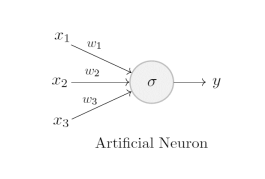
\includegraphics[width = 3in]{images/artificialneuron.png}
	\caption{Artificial Neuron} %figure name
	\label{figArtificialNeuron} % for referencing
\end{center}
\end{figure}

The network consists of connections, each connection providing the output of one
neuron as an input to another neuron. Each connection is assigned a weight that
represents its relative importance. A given neuron can have multiple input and
output connections.\\
The neurons are typically organized into multiple layers, especially in deep
learning. Neurons of one layer connect only to neurons of the immediately
preceding and immediately following layers. The layer that receives external data
is the input layer. The layer that produces the ultimate result is the output layer. In
between them are zero or more hidden layers.

\begin{figure}[tbh] % tbh means top, bottom or here (priority: left to right)
\begin{center}
	%
\includegraphics[width = 3in]{images/logo.png}
	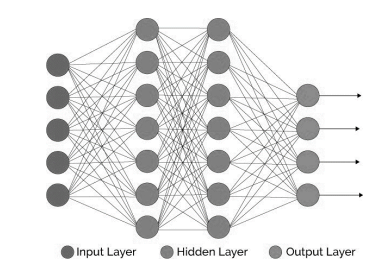
\includegraphics[width = 3in]{images/structure.png}
	\caption{Structure of Neural Network} %figure name
	\label{figStructure of Neural Network} % for referencing
\end{center}
\end{figure}

\subsection{Convolutional Neural Network(CNN)}
CNN is a kind of neural network, its weight sharing network structure makes it more similar to the
biological neural network, reduces the complexity of the network model and the
number of weights [5].CNNs were inspired by biological processes. The name
“convolutional neural network” indicates that the network employs a
mathematical operation called convolution. Convolution is a specialized kind of
linear operation. They use convolution in place of general matrix multiplication in at least one of their layers.

\subsubsection{Design}
A convolutional neural network consists of an input and an output layer, as well as multiple hidden layers. The hidden layers of a CNN typically consist of a series of convolutional layers that convolve with a multiplication or other dot product.
\pagebreak

\begin{figure}[tbh] % tbh means top, bottom or here (priority: left to right)
\begin{center}
	%
\includegraphics[width = 3in]{images/logo.png}
	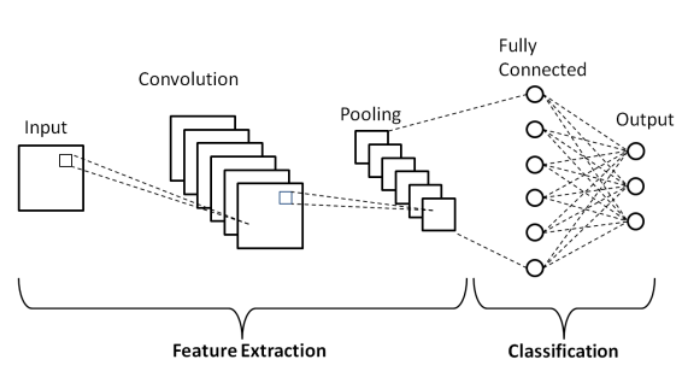
\includegraphics[width = 5in]{images/cnn.png}
	\caption{Basic schematic of Convolutional Neural Network(CNN)} %figure name
	\label{figStructure of Neural Network} % for referencing
\end{center}
\end{figure}

A CNN typically has three layers:

\begin{itemize}
\item Convolutional layer:This layer performs a dot product between two matrices, where one matrix is the set of learnable parameters otherwise known as a kernel, and the other matrix is the restricted portion of the receptive field. The kernel is spatially smaller than an image but is more in-depth. This means that, if the image is composed of three (RGB) channels, the kernel height and width will be spatially small, but the depth extends up to all three channels.During the forward pass, the kernel slides across the height and width of the image-producing the image representation of that receptive region. This produces a two-dimensional representation of the image known as an activation map that gives the response of the kernel at each spatial position of the image. The sliding size of the kernel is called a stride.

\begin{figure}[htb] % tbh means top, bottom or here (priority: left to right)
\begin{center}
	%
\includegraphics[width = 3in]{images/logo.png}
	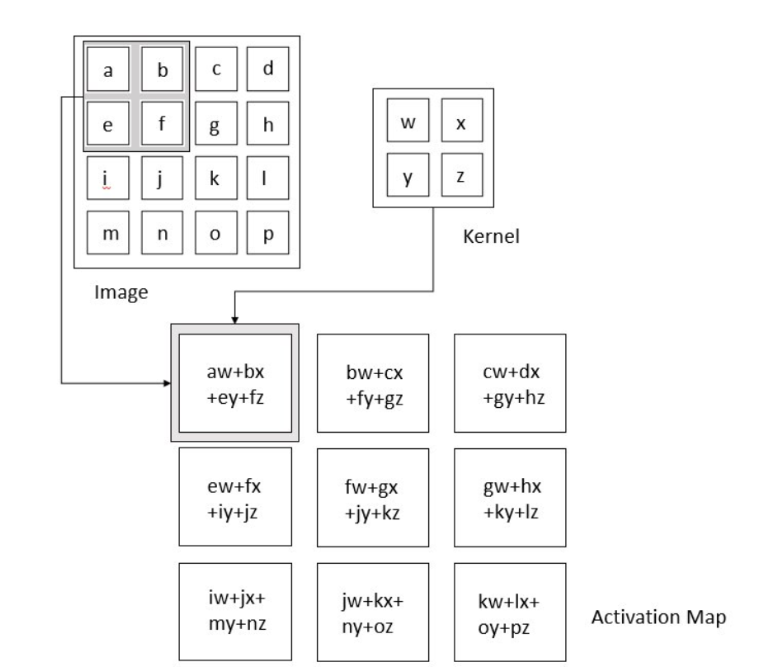
\includegraphics[width = 2in]{images/activationmap.png}
	\caption{Activation Map} %figure name
	\label{figActivationMap} % for referencing
\end{center}
\end{figure}

\item Pooling layer: The pooling layer replaces the output of the network at certain locations by deriving a summary statistic of the nearby outputs. This helps in reducing the spatial size of the representation, which decreases the required amount of computation and weights. The pooling operation is processed on every slice of the representation individually.

\begin{figure}[htb] % tbh means top, bottom or here (priority: left to right)
\begin{center}
	%
\includegraphics[width = 3in]{images/logo.png}
	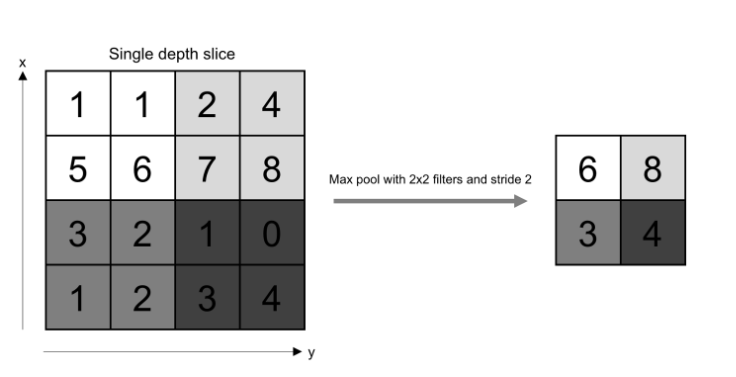
\includegraphics[width = 4in]{images/pooling.png}
	\caption{Pooling Operation} %figure name
	\label{figPoolingOperation} % for referencing
\end{center}
\end{figure}

\item Fully connected layer: Neurons in this layer have full connectivity with all neurons in the preceding and succeeding layer as seen in regular Forward Convolutional Neural Network(FCNN). This is why it can be computed as usual by a matrix multiplication followed by a bias effect.
\end{itemize}

\subsection{Hough Transform}
The Hough transform (HT) was firstly proposed in for machine analysis of bubble chamber photographs. It parametrizes straight lines with slope-offset, leading to an unbounded transform space (since the slope can be infinity). extended HT by using angle-radius rather than slope-offset parameters, and is conceptually similar to two-dimensional Radom transform. Then generalized the idea of HT to localize arbitrary shapes, e.g. ellipses and circles, from digital images. For example, by parameterizing with angle and radius, line detection can be performed by voting edge evidence and finding peak response in the finite parametric space. Typically, with the edge detectors such as Canny  and Sobel , the detected lines are the maximal local response points in the transformed parametric space. The core idea of HT is used in two recent works which parameterize the outputs of CNNs with offsets and orientations to predict surface meshes  or convex decomposition  of 3D shapes. Despite the success of HT on line detection, it suffers from high computational costs and unstable performance. To accelerate the voting of HT proposed the “probabilistic Hough transform” to randomly pick sample points from a line, while  using the gradient direction of images to decide the voting points. Meanwhile, the work of employed kernel-based Hough transform to perform hough voting by using the elliptical-Gaussian kernel on collinear pixels to boost the original HT. Besides partitioned the input image into hierarchical image patches, and then applied HT independently to these patches. Use a coarse-to-fine accumulation and search strategy to identify significant peaks in the Hough parametric spaces. tackled line detection within a regularized framework, to suppress the effect of noise and clutter corresponding to nonlinear image features. The Hough voting scheme is also used in many other tasks such as detecting centroid of 3D shapes in point cloud and finding image correspondence.

\chapter{Methodology}
Automatic driving license consists of two parts. Object detection and lane detection. Object detection will be used to determine the position of vehicle and the position obtained will be compared with lane. If the position of vehicle is determined to be touching the lane then test will be automatically stopped prompting a message.  

%Flow Chart of system
\begin{figure}[tbh] % tbh means top, bottom or here (priority: left to right)
\begin{center}
	%
\includegraphics[width = 3in]{images/logo.png}
	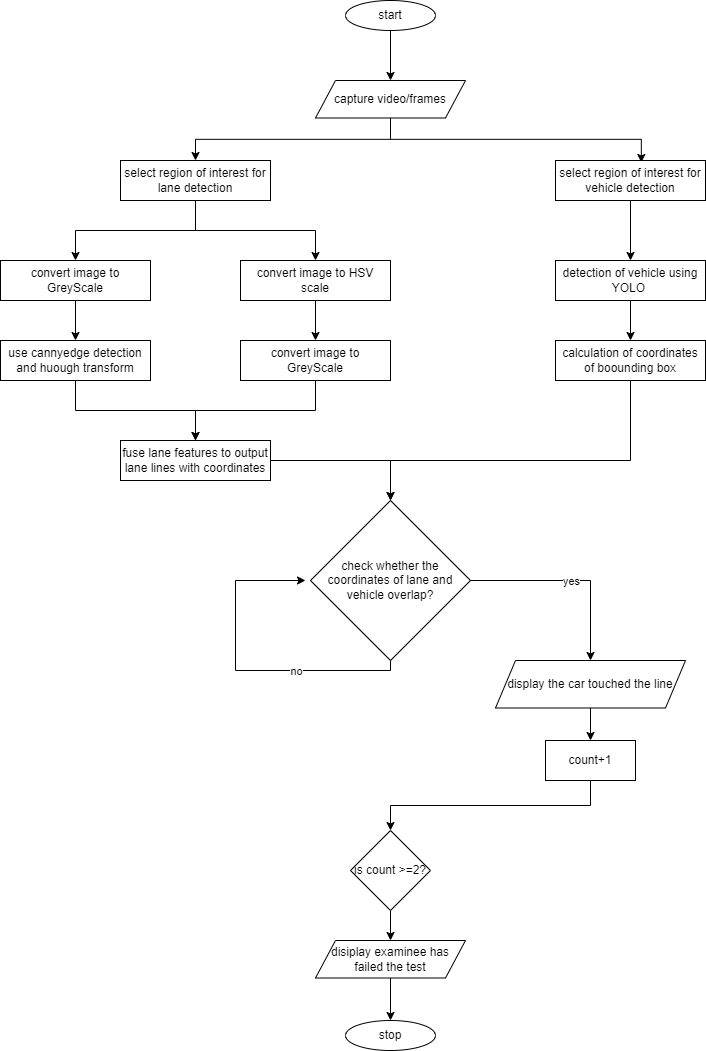
\includegraphics[width = 4in]{images/system flowchart changed.png}
	\caption{Flow chart of System} %figure name
	\label{figObjectDetectionusingYOLO} % for referencing
\end{center}
\end{figure}

%Block diagram of system
\begin{figure}[tbh] % tbh means top, bottom or here (priority: left to right)
\begin{center}
	%
\includegraphics[width = 3in]{images/logo.png}
	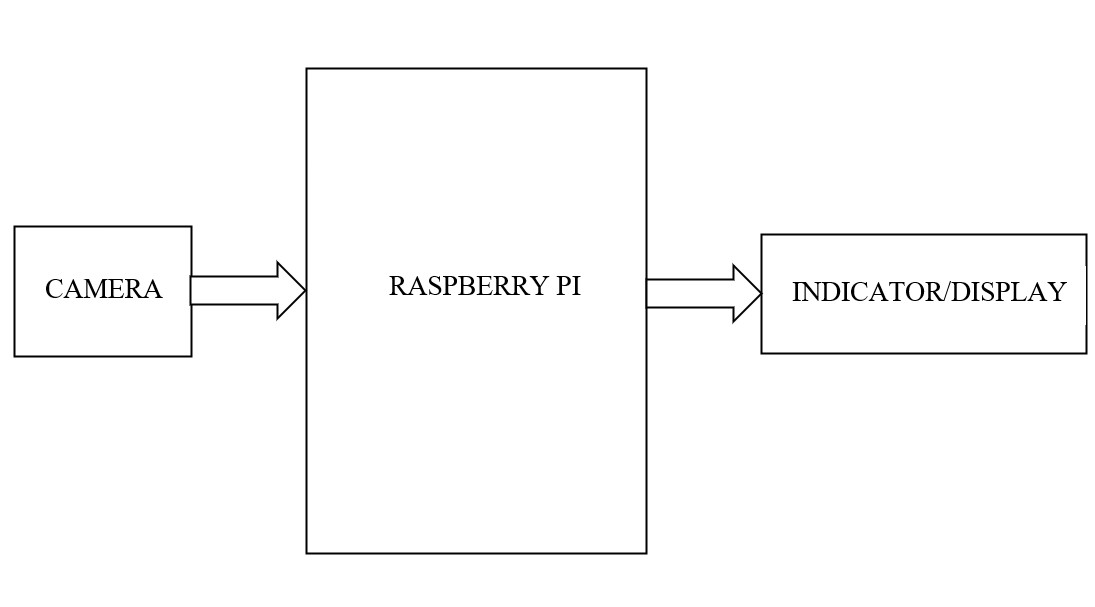
\includegraphics[width = 4in]{images/block diagram of system.jpg}
	\caption{Block Diagram of System} %figure name
	\label{figObjectDetectionusingYOLO} % for referencing
\end{center}
\end{figure}



\section{Object Detection}
The Object Detection part focuses on detecting the car body precisely using You Only Look Once(YOLO) algorithm. \\

\begin{figure}[tbh] % tbh means top, bottom or here (priority: left to right)
\begin{center}
	%
\includegraphics[width = 3in]{images/logo.png}
	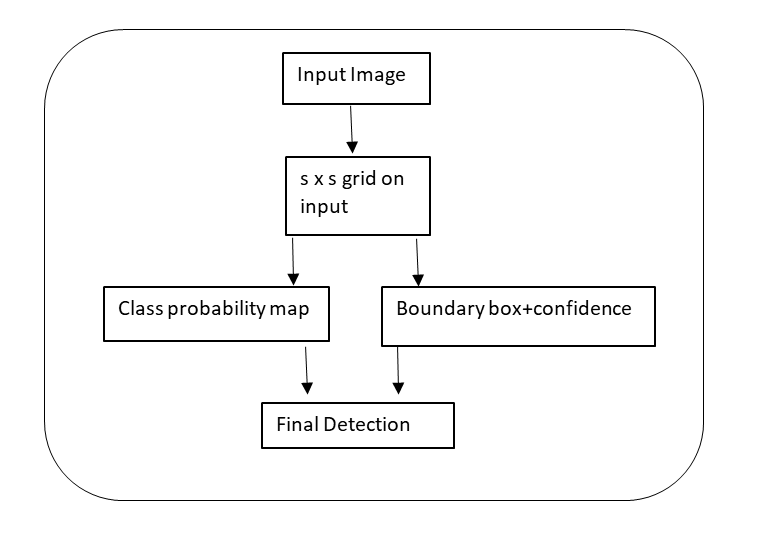
\includegraphics[width = 4in]{images/yolo.png}
	\caption{Object detection using YOLO} %figure name
	\label{figObjectDetectionusingYOLO} % for referencing
\end{center}
\end{figure}

You Only Look Once(YOLO) algorithm works using the following three techniques:

\begin{itemize}
\item Residual blocks:First, the image is divided into various grids. Each grid has a dimension of S x S.Every grid cell will detect objects that appear within them.
\item Bounding box regression: A bounding box is an outline that highlights an object in an image.Every bounding box in the image consists of the attributes, width (bw), height (bh), class, bounding box center (bx,by).
\item Intersection Over Union (IOU):Intersection over union (IOU) is a phenomenon in object detection that describes how boxes overlap. YOLO uses IOU to provide an output box that surrounds the objects perfectly.
\end{itemize}

\section{Lane Detection}
Hough transform is a feature extraction method used in image analysis. The purpose of the technique is to find imperfect instances of objects within a certain class of shapes by a voting procedure. This voting procedure is carried out in a parameter space, from which object candidates are obtained as local maxima in a so-called accumulator space that is explicitly constructed by the algorithm for computing the Hough transform. Hough transform can be used to isolate features of any regular curve like lines, circles, ellipses, etc. Hough transform in its simplest from can be used to detect straight lines in an image. A generalized Hough transform can be used in applications where simple analytic description of features is not possible. 

\begin{figure}[H] % tbh means top, bottom or here (priority: left to right)
\begin{center}
	%
\includegraphics[width = 3in]{images/logo.png}
	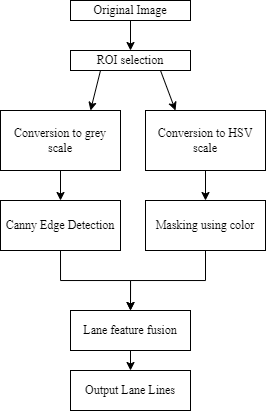
\includegraphics[height = 4in]{images/lane detection.png}
	\caption{Lane Detection using feature selection} %figure name
	\label{figLaneDetectionusingFeatureSelection} % for referencing
\end{center}
\end{figure}

\subsection{Testing}
Effectiveness of the software will be tested by building a scaled downed model. The scaled downed car is in ratio 0f 1:17 with real car.
%Block diagram of car
\begin{figure}[H] % tbh means top, bottom or here (priority: left to right)
\begin{center}
	%
\includegraphics[width = 3in]{images/logo.png}
	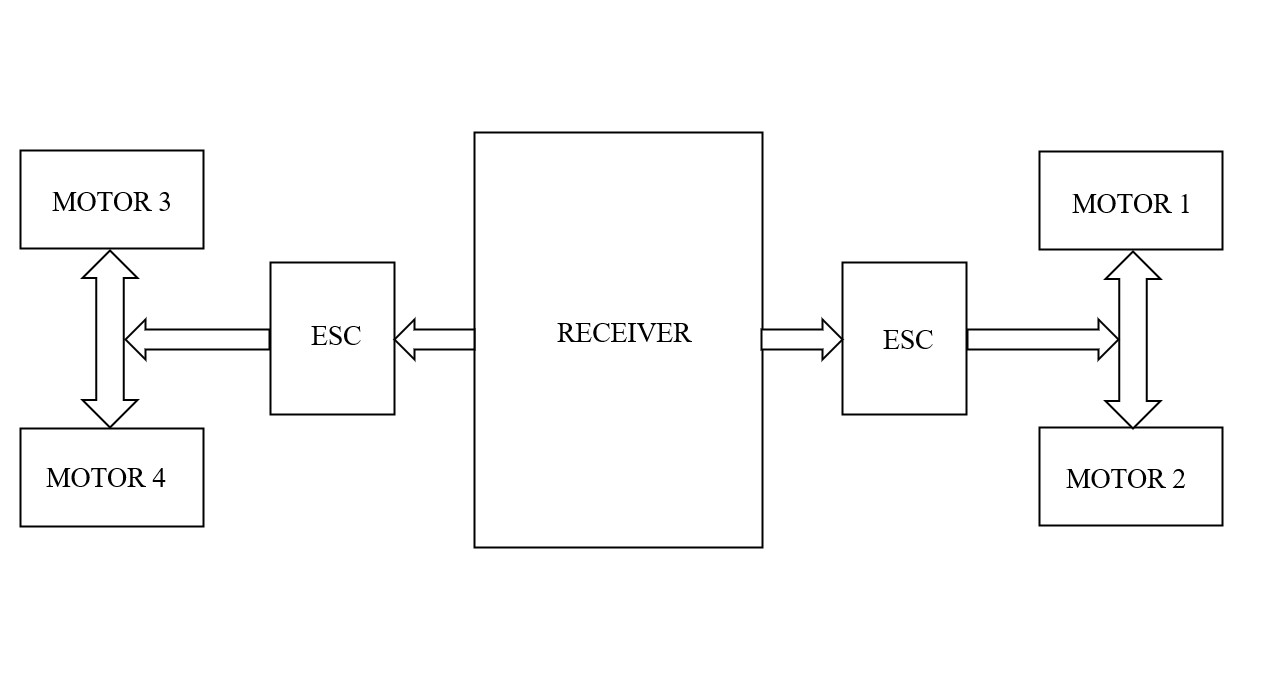
\includegraphics[width = 4in]{images/block diagram of car.jpg}
	\caption{Block Diagram of Car} %figure name
	\label{figObjectDetectionusingYOLO} % for referencing
\end{center}
\end{figure}

Four motor are used in the scaled down model of the car. The motors are controlled using Electronics Speed Controller(ESC) and control signal is provided to the Electronic Speed Controller through a 2.4 Ghz receiver. A 2.4 Ghz transmitter is used by controller to transmit control signal wirelessly. 

\chapter{Epilogue}

\section{Work Completed}
As part of the "Automated Driving License Test" project, we have made significant progress in developing a software solution for administering driving license exams. The following tasks and milestones have been completed:
\begin{enumerate}
\item Scaled downed car: A scaled down version of test car with four wheels is constructed to test the software's performance.  
\item Custom object detection: Software if able to identify scaled down test car with accuracy of 0.9.
\item Lane Detection: An algorithm for the detection of road lines is developed and is in the process of refinement to increase it's accuracy and 	reliability. 
\item Pass or Fail determination: CNN is able to identify if the car has touched the line or not and is able to determine whether the examinee has passed or failed the exam. 
\end{enumerate}


\section{Work in Process}
\begin{enumerate}
\item Lane detection is on process of refinement.
\item Data model training.
\item Scaled downed Track.
\item Linking all algorithms into one program.
\end{enumerate}

\section{Work Remaining}
\begin{enumerate}
\item Scaled downed Track.
\item Linkning all algorithms into one program
\end{enumerate}
   
%\hline
\section{Result}
\begin{enumerate}
\item The system predicts that the examinee has failed their exam when the robot touches the line
\begin{figure}[H] % tbh means top, bottom or here (priority: left to right)
\begin{center}
	%
\includegraphics[width = 3in]{images/logo.png}
	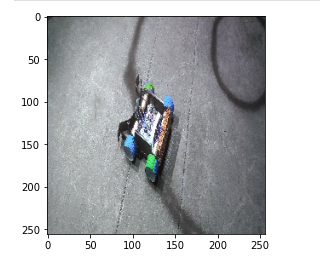
\includegraphics[width = 3in]{images/linet.png}
	 %figure name
	\label{figSample1} % for referencing
\end{center}
\end{figure}
\begin{figure}[H] % tbh means top, bottom or here (priority: left to right)
\begin{center}
	%
\includegraphics[width = 3in]{images/logo.png}
	
\includegraphics[width = 2in]{images/linetr.png}
	\caption{example of result prediction} %figure name
	\label{figSample1} % for referencing
\end{center}
\end{figure}
\item The system predicts that the examinee has passed their exam when the robot does not touch the line
\begin{figure}[H] % tbh means top, bottom or here (priority: left to right)
\begin{center}
	%
\includegraphics[width = 3in]{images/logo.png}
	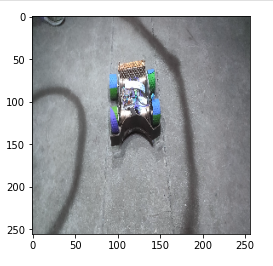
\includegraphics[width = 3in]{images/linent.png}
	 %figure name
	\label{figSample1} % for referencing
\end{center}
\end{figure}
\begin{figure}[H] % tbh means top, bottom or here (priority: left to right)
\begin{center}
	%
\includegraphics[width = 3in]{images/logo.png}
	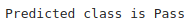
\includegraphics[width = 2in]{images/linentr.png}
	\caption{example of result prediction} %figure name
	\label{figSample1} % for referencing
\end{center}
\end{figure}
\item 
\begin{figure}[H] % tbh means top, bottom or here (priority: left to right)
\begin{center}
	%
\includegraphics[width = 3in]{images/logo.png}
	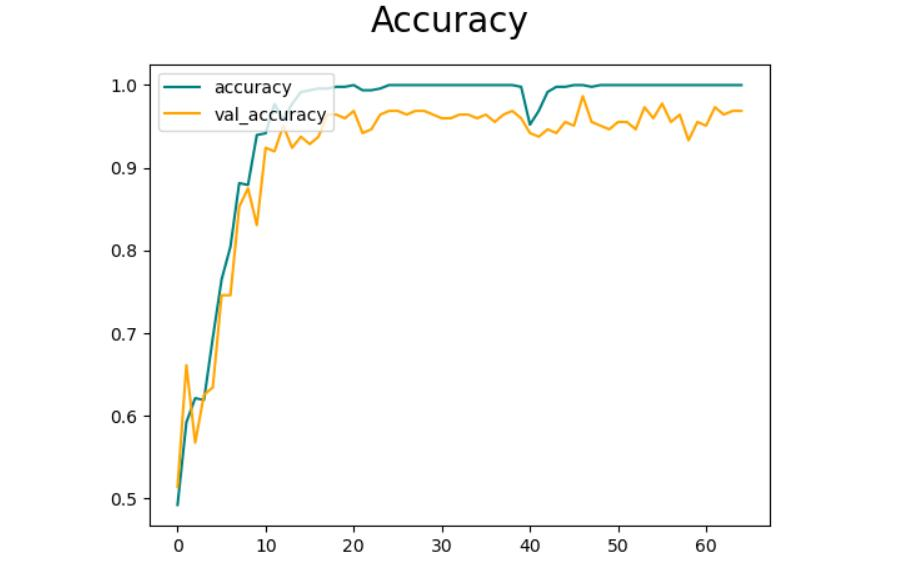
\includegraphics[width = 4in]{images/accuracy65epoch.jpg}
	 \caption{Accuracy} %figure name
	\label{figSample1} % for referencing
\end{center}
\end{figure}
\item 
\begin{figure}[H] % tbh means top, bottom or here (priority: left to right)
\begin{center}
	%
\includegraphics[width = 3in]{images/logo.png}
	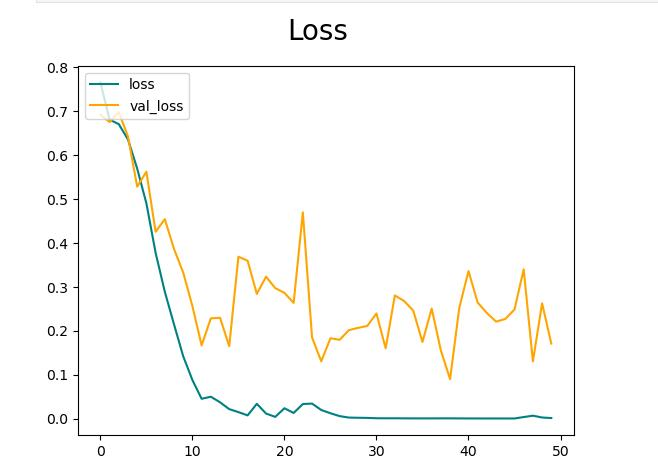
\includegraphics[width = 4in]{images/loss.jpg}
	 \caption{Loss} %figure name
	\label{figSample1} % for referencing
\end{center}
\end{figure}
\item 
\begin{figure}[H] % tbh means top, bottom or here (priority: left to right)
\begin{center}
	%
\includegraphics[width = 3in]{images/logo.png}
	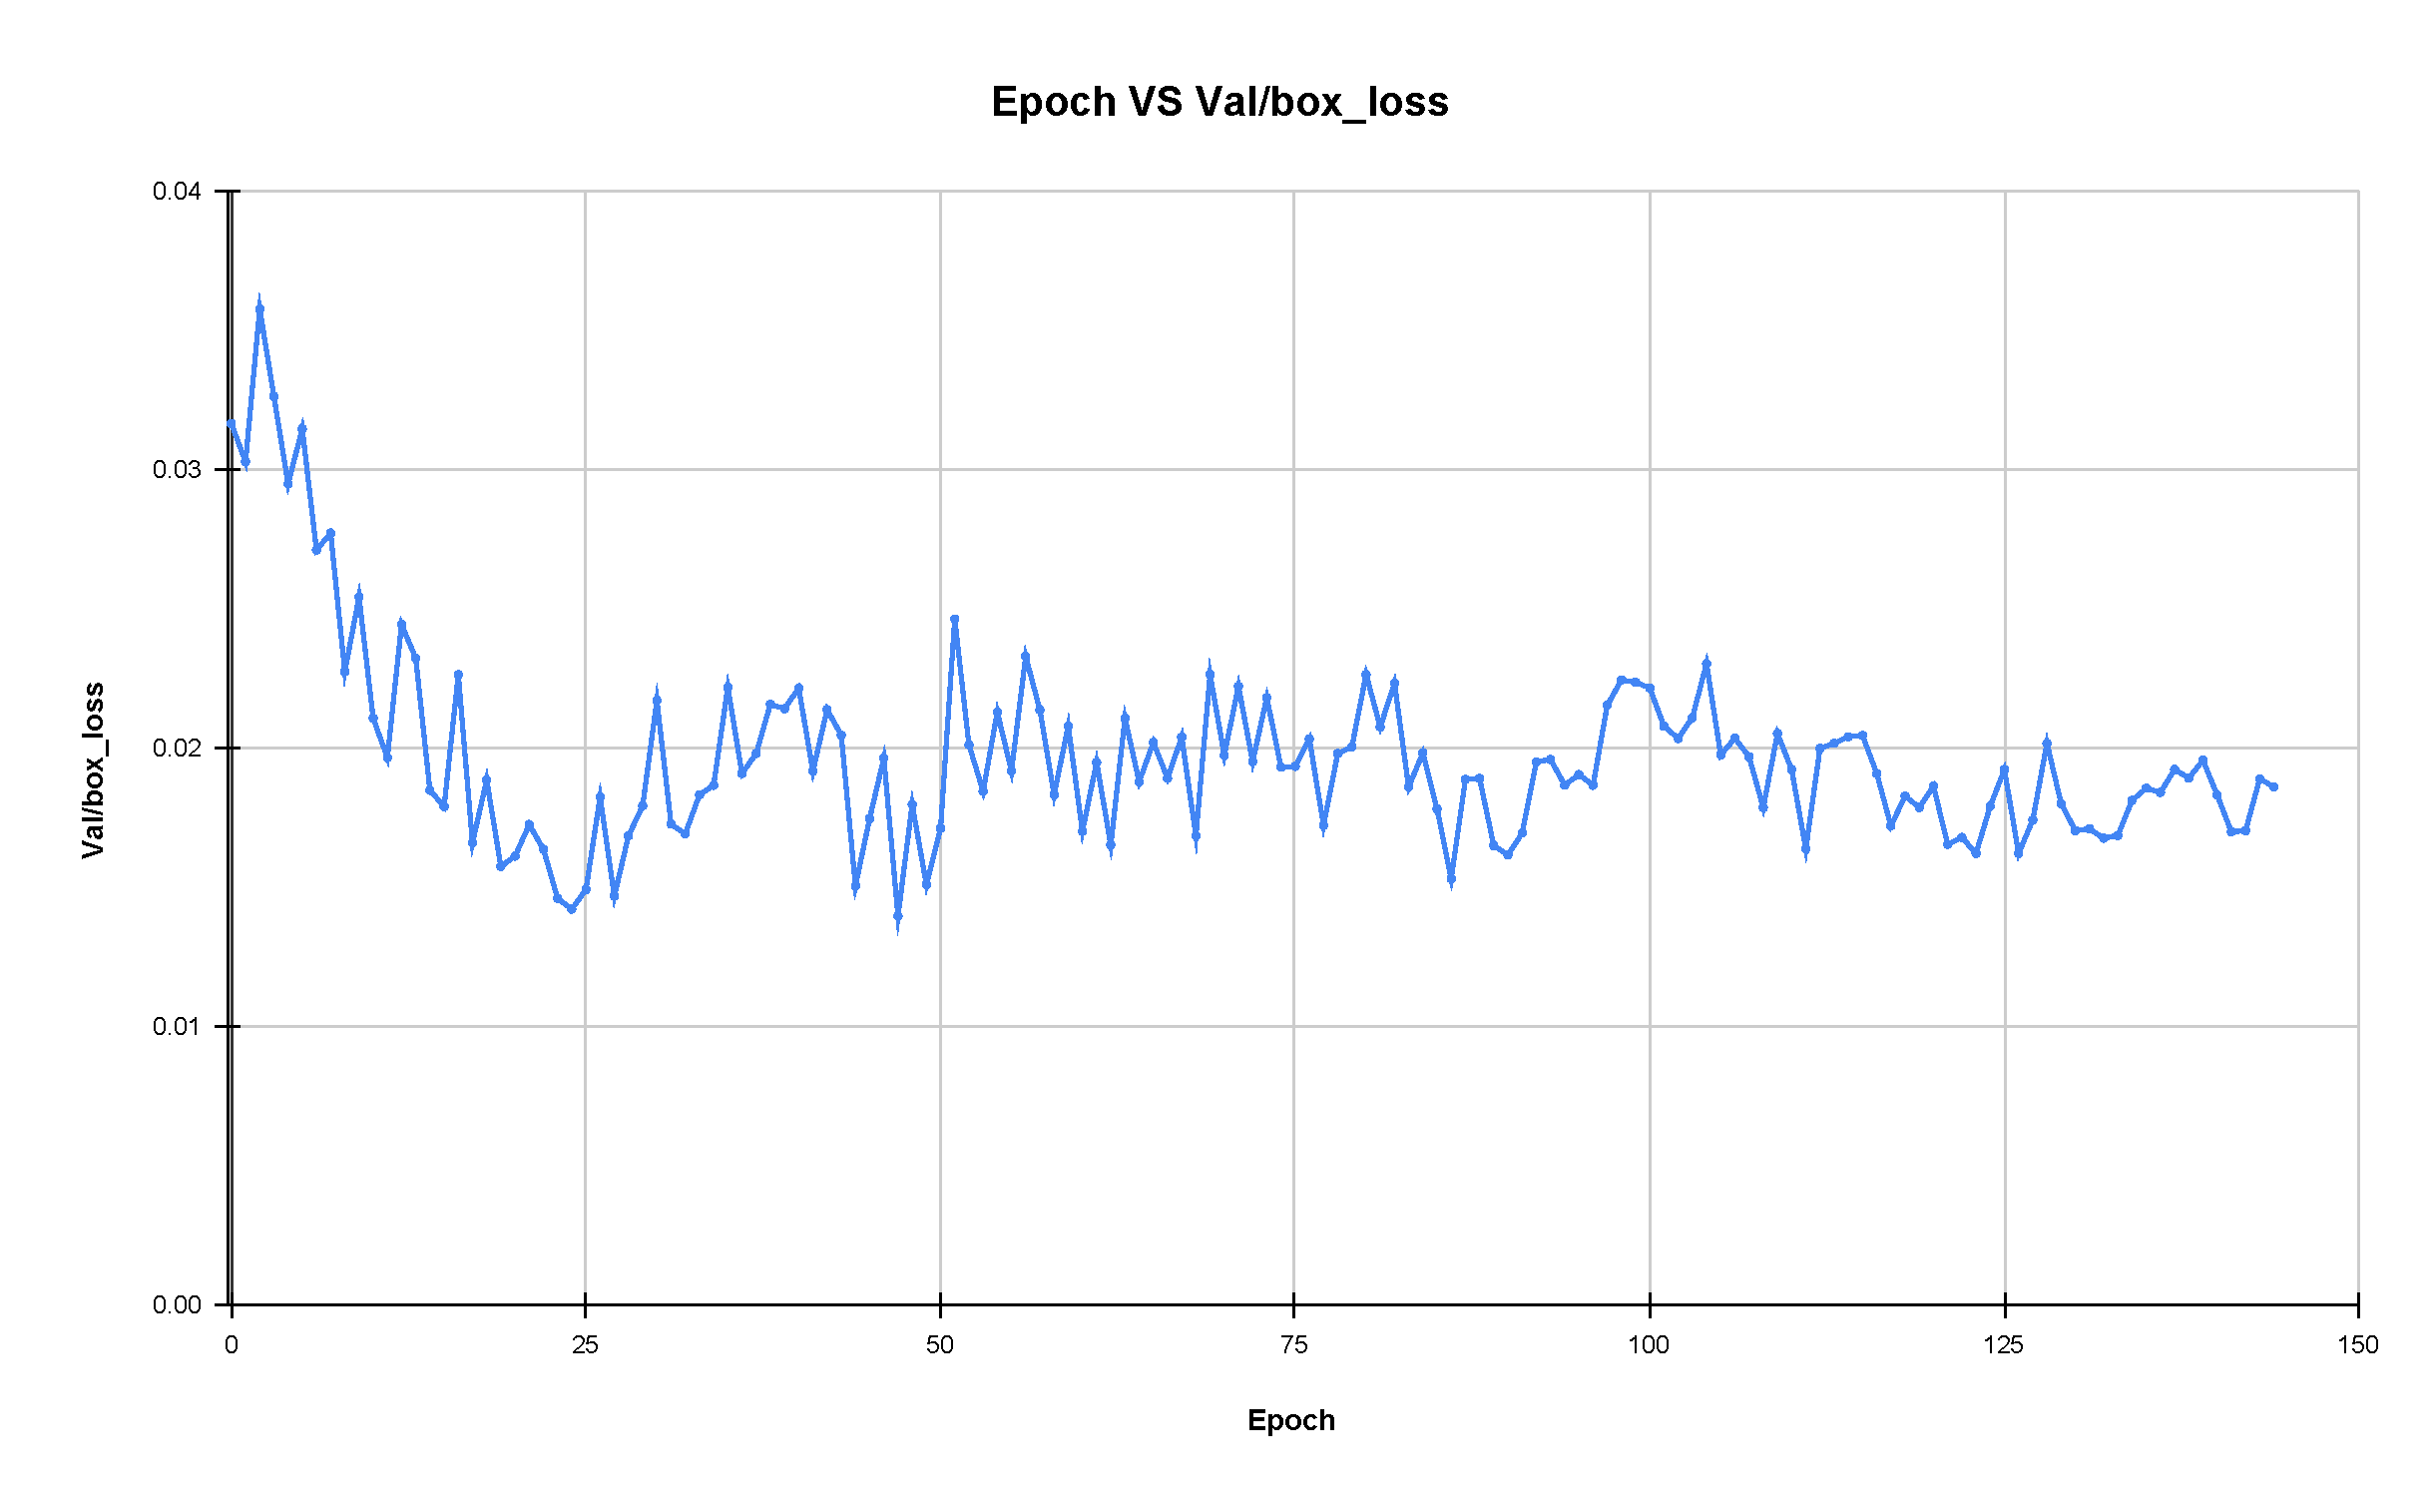
\includegraphics[width = 4in]{images/Epoch VS Val_box_loss.pdf}
	 \caption{Epoch VS Val box loss for YOLO} %figure name
	\label{figSample1} % for referencing
\end{center}
\end{figure}
\item 
\begin{figure}[H] % tbh means top, bottom or here (priority: left to right)
\begin{center}
	%
\includegraphics[width = 3in]{images/logo.png}
	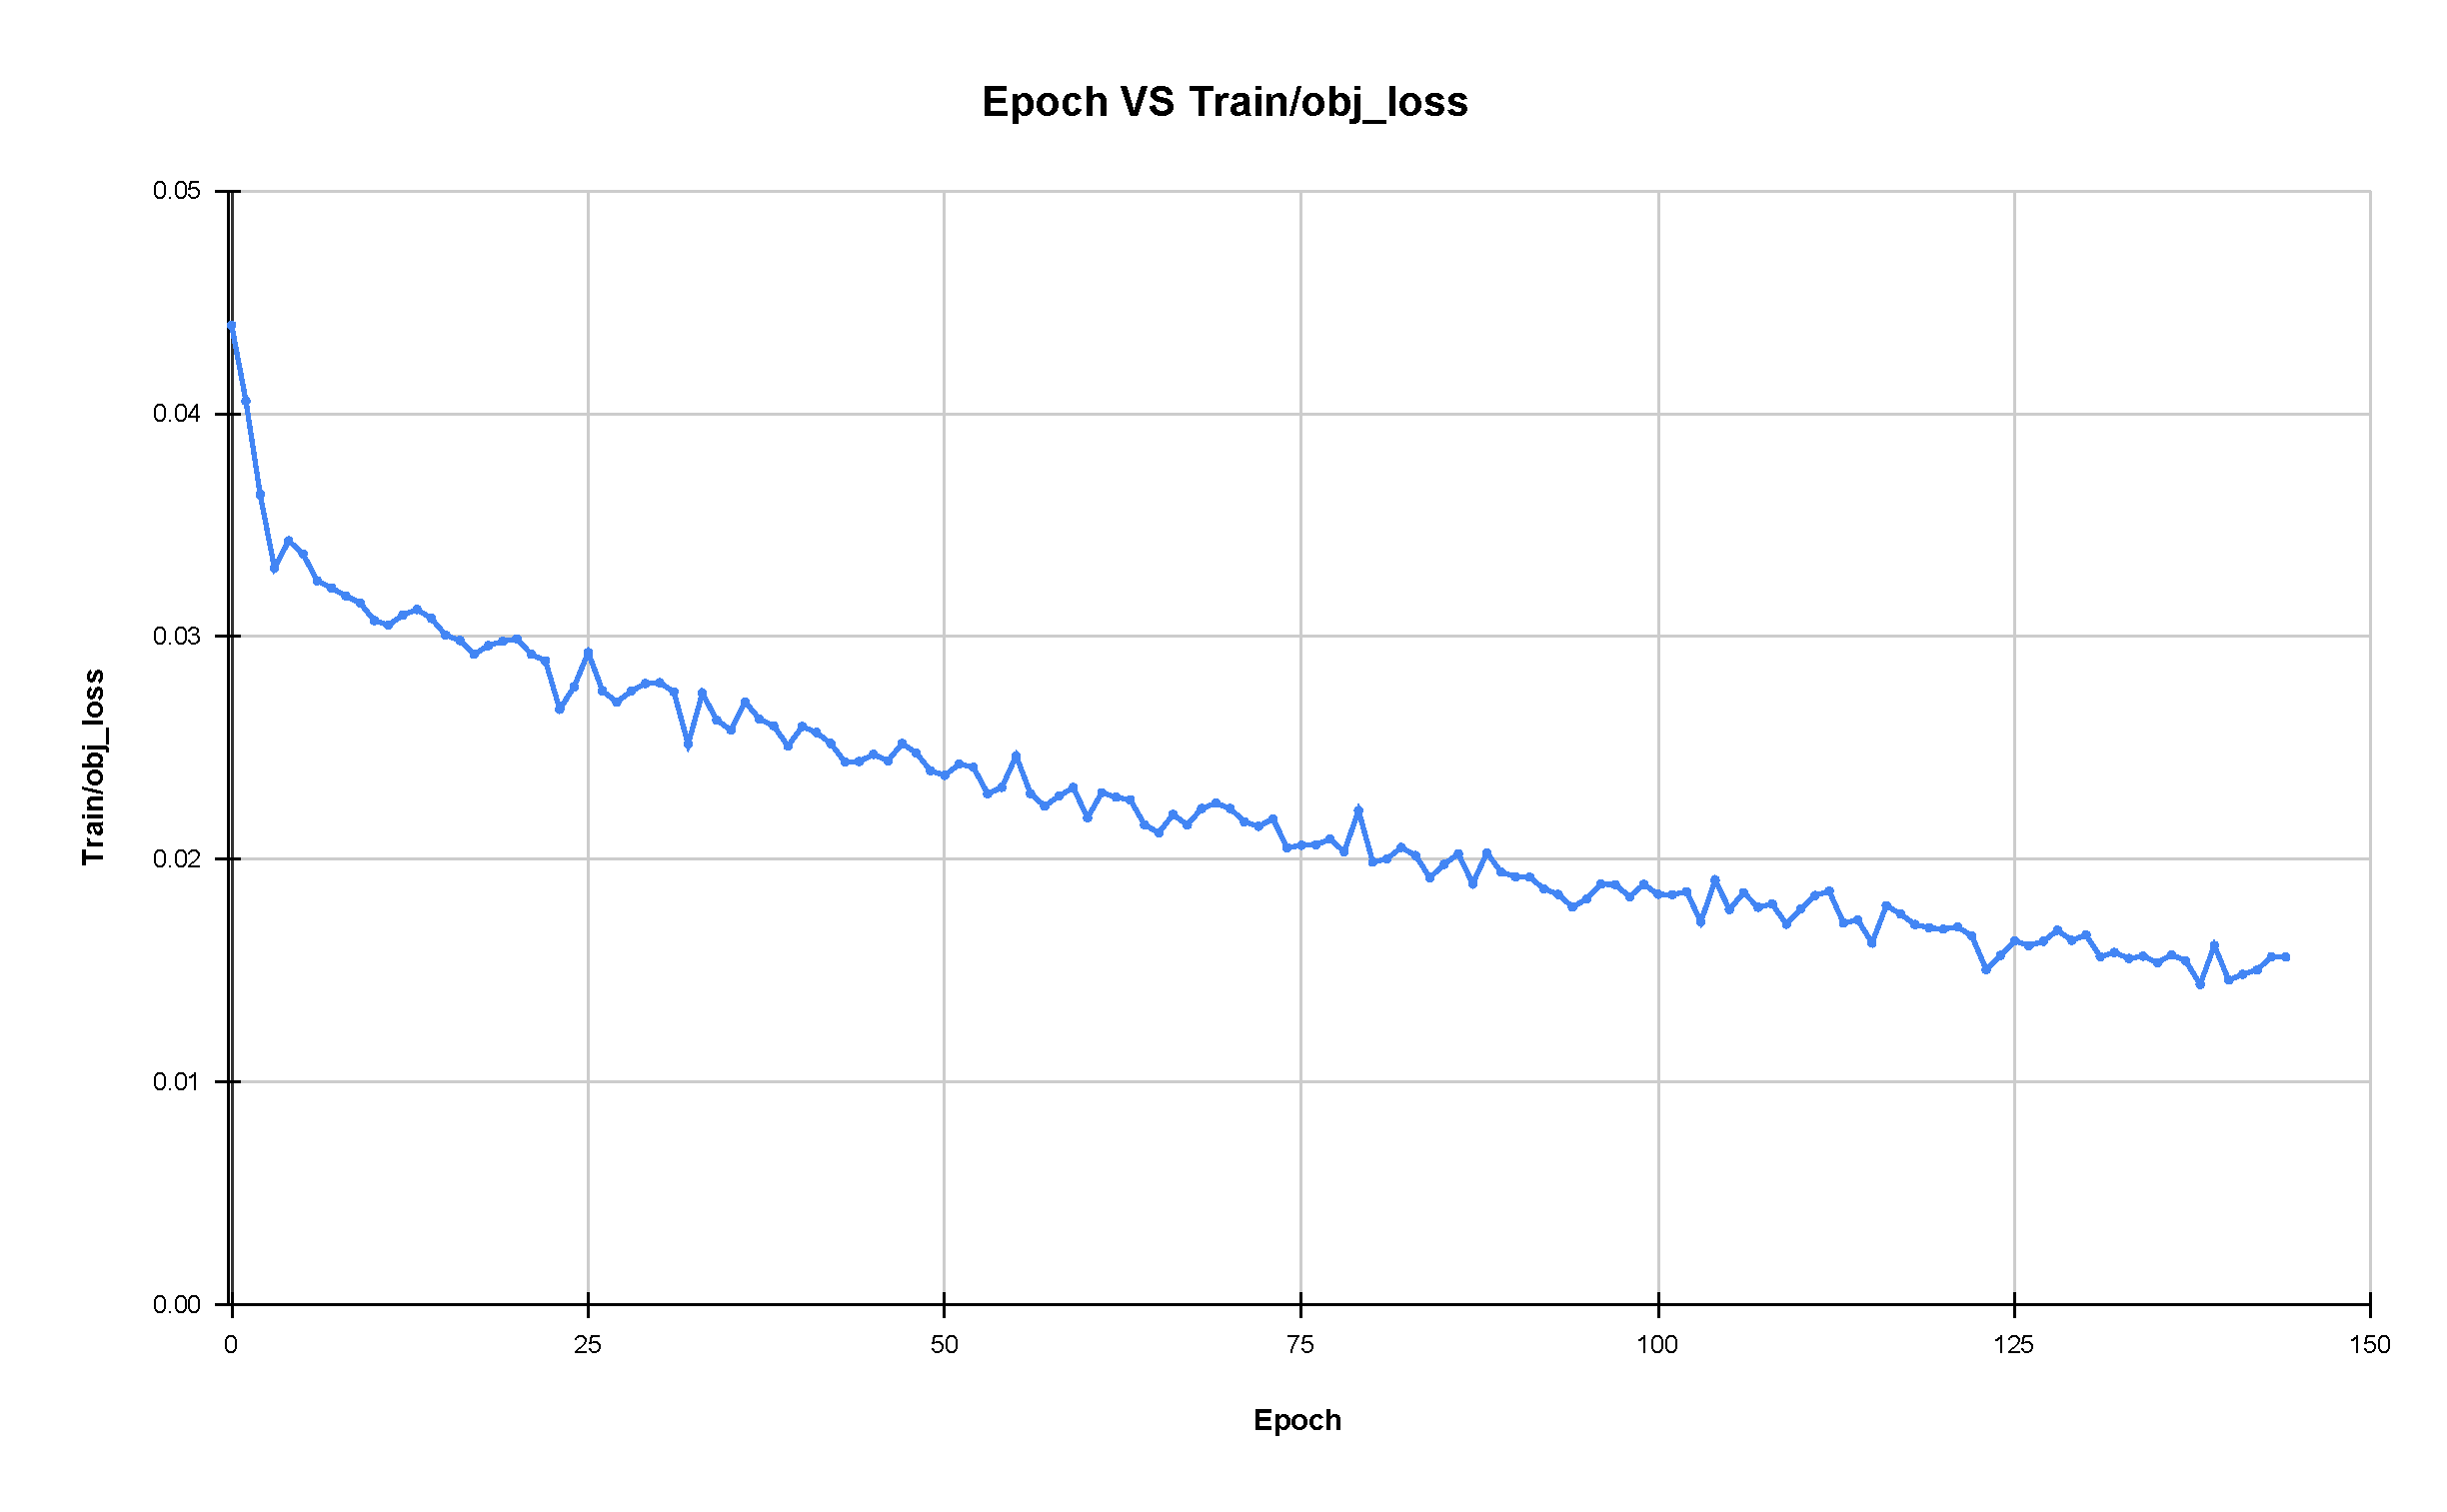
\includegraphics[width = 4in]{images/Epoch VS Train_obj_loss.pdf}
	 \caption{Epoch VS Train obj loss for YOLO} %figure name
	\label{figSample1} % for referencing
\end{center}
\end{figure}
\end{enumerate}


\section{Work Scheduled}

\begin{figure}[H] % tbh means top, bottom or here (priority: left to right)
\begin{center}
	%
\includegraphics[width = 3in]{images/logo.png}
	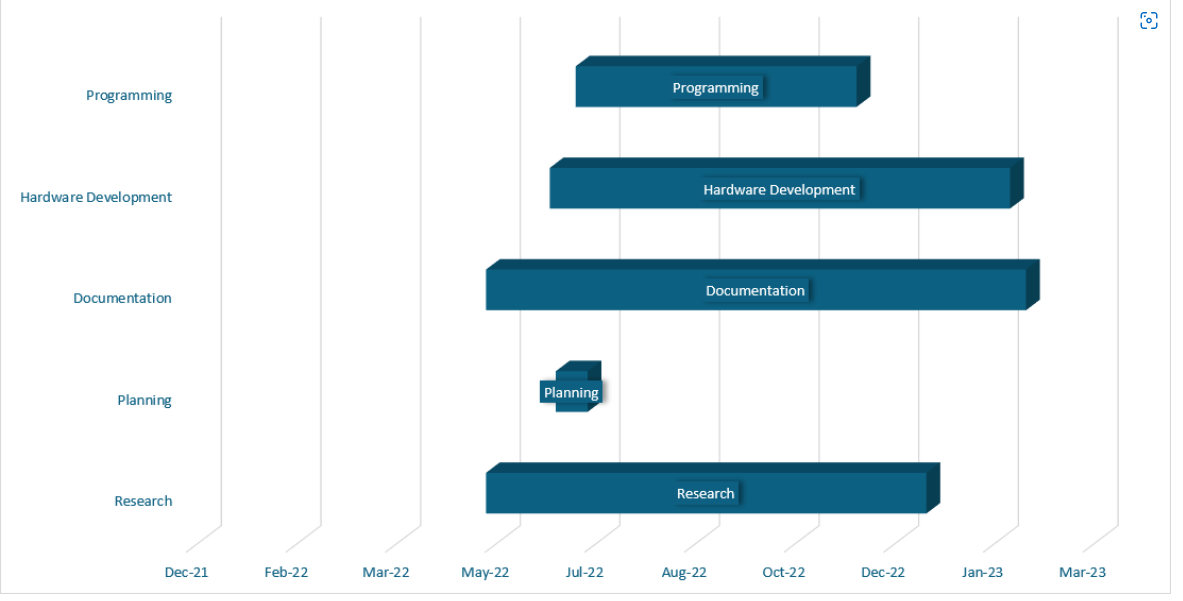
\includegraphics[width = 7in]{images/ganttchart.png}
	\caption{Gantt Chart} %figure name
	\label{figSample1} % for referencing
\end{center}
\end{figure}

\section{Cost Estimation}

\begin{table}[H]
\centering
\begin{tabular}{|l|c|c|c|c|} %c,l,r represent alignment, number of c,l or r represent number of columns, | for Vertical line
	\hline %horizontal line
	\multicolumn{1}{|c|}{Items}  &No. of Item &Unit Price(Rs.) &Total Price(Rs.)\\
	\hline %horizontal line
	Raspberry Pi 4 &2 &4,500/- &9,000/-\\
	\hline %horizontal line
	200 rpm metal gear dc motor &4 &1000/- &4000/-\\
	\hline
	Arduino Nano &1 &800/- &800/-\\
	\hline
	Motor Driver Module &2 &1000/- &2000/-\\
	\hline
	RTC module &1 &200/- &200/-\\
	\hline
	Pi camera/ USB camera &2 &1500/- &3000/-\\
	\hline
	Bluetooth Module &1 &800/- &800/-\\
	%\hline
	%Flex Sensor &4 &300/- &1200/-\\
	\hline
	\multicolumn{3}{|c|}{Total} &21,000/-\\
	\hline
\end{tabular}

\caption{Cost Estimation}

\label{tblCostEstimationTable}
\end{table}


%\chapter{}
\subsubsection{Snapshots}
\subsubsection{Work Done}
\begin{figure}[!th] % tbh means top, bottom or here (priority: left to right)
%\begin{centre}
	%
\includegraphics[width = 3in]{images/logo.png}
	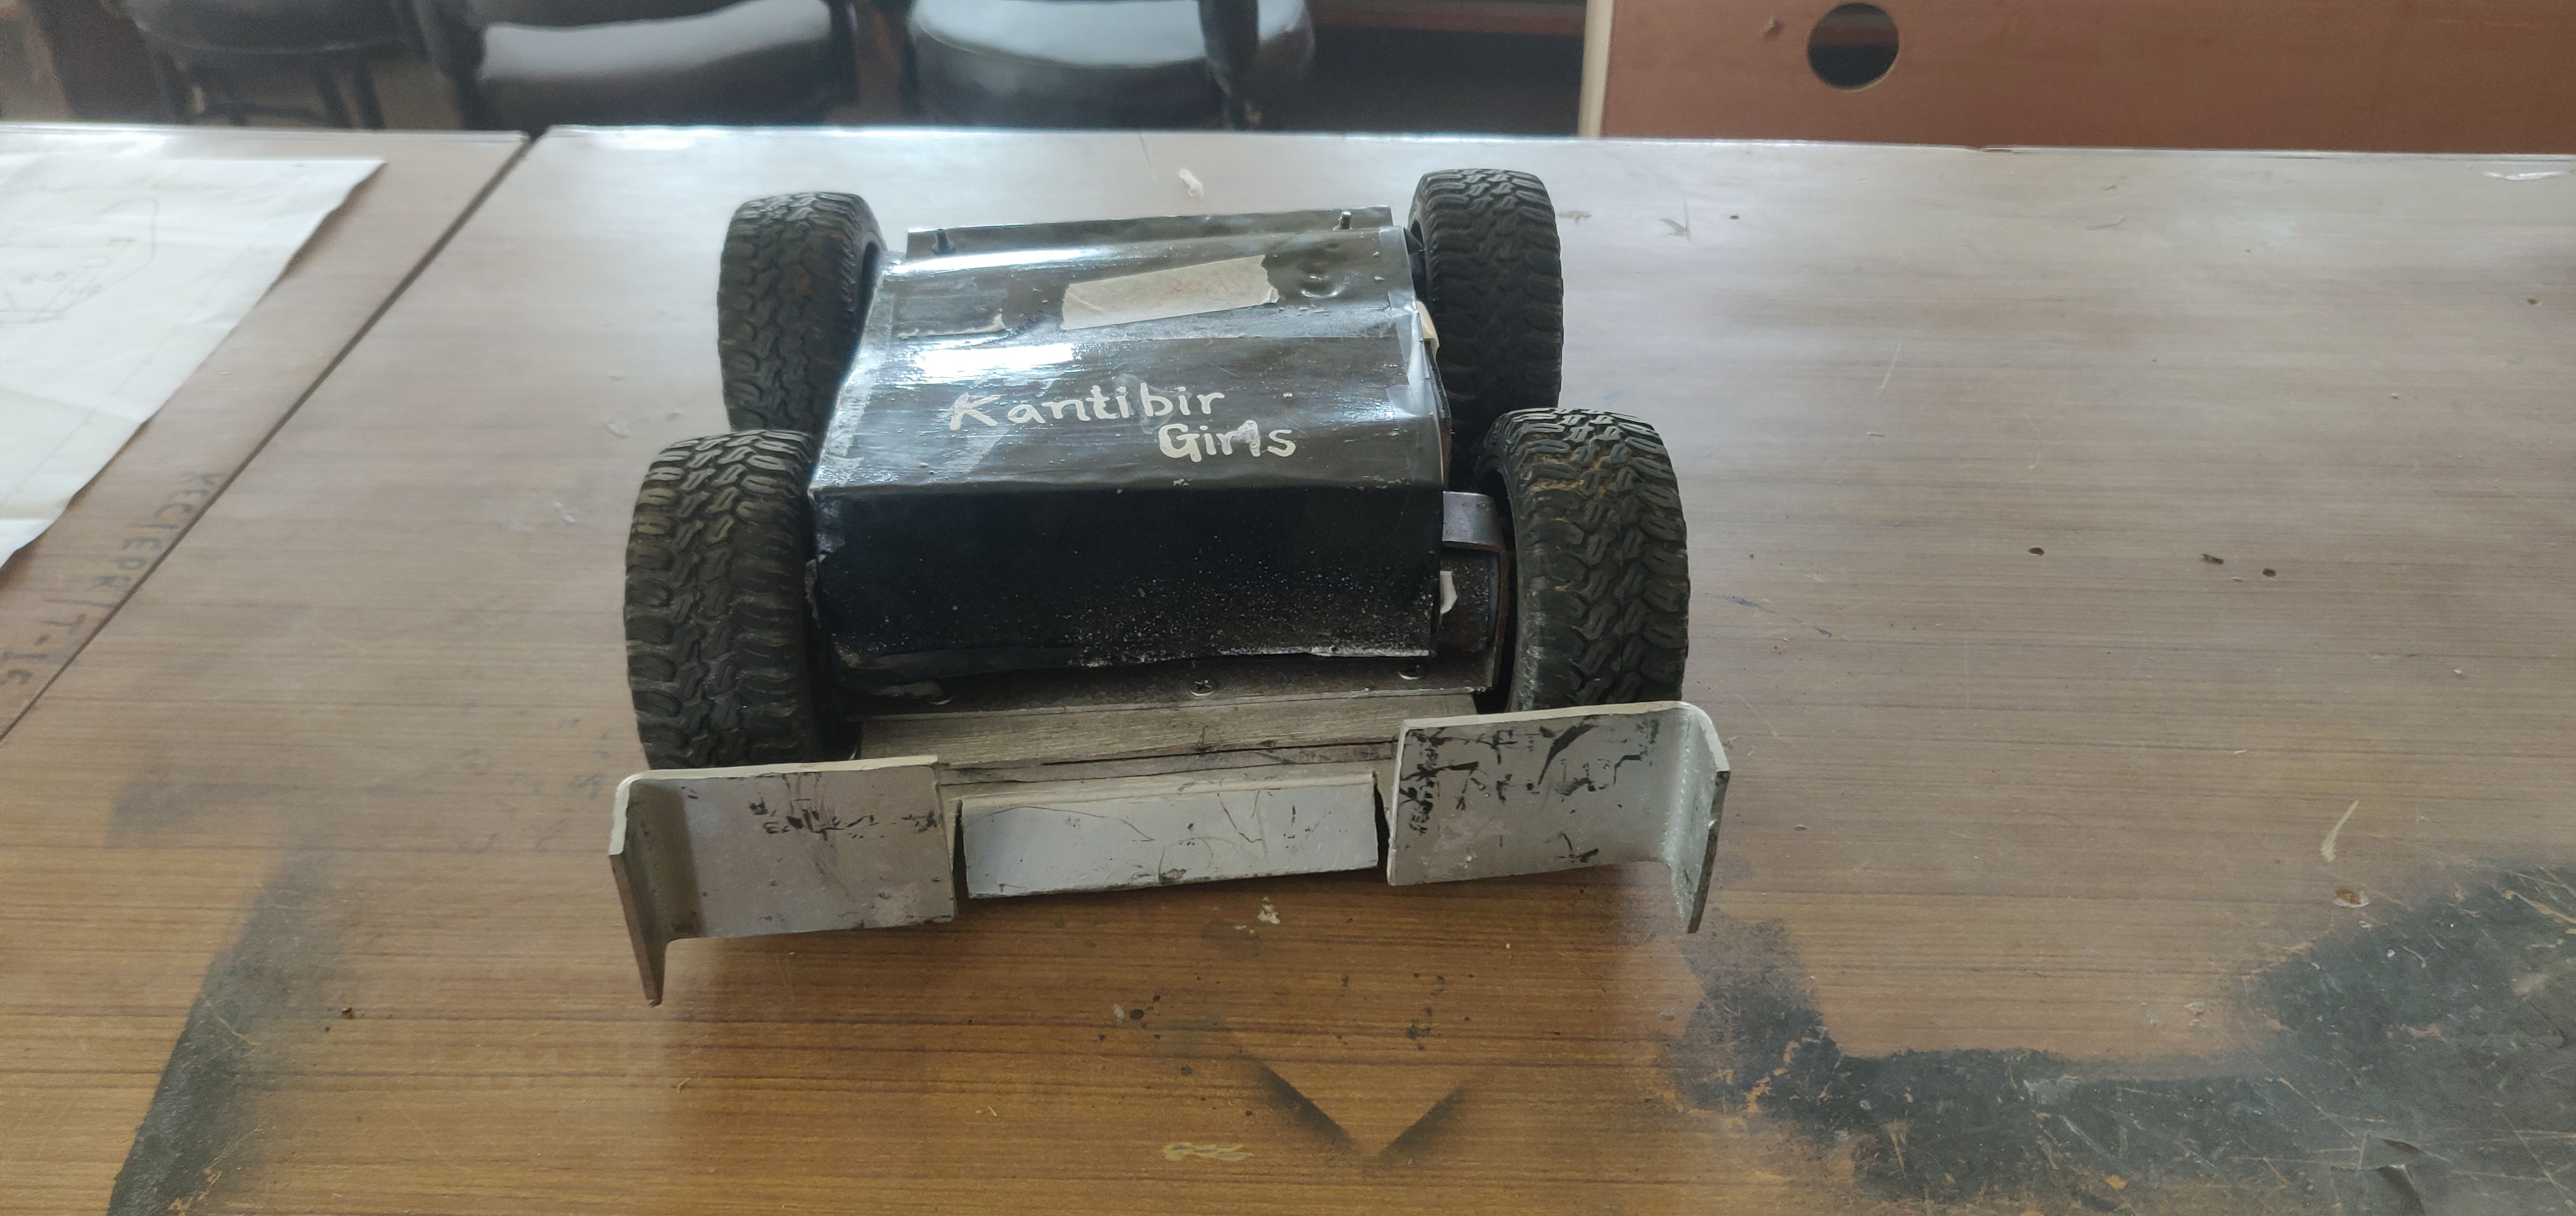
\includegraphics[width = 3in]{images/botpic10.jpg} 
	\hspace{.5cm}
	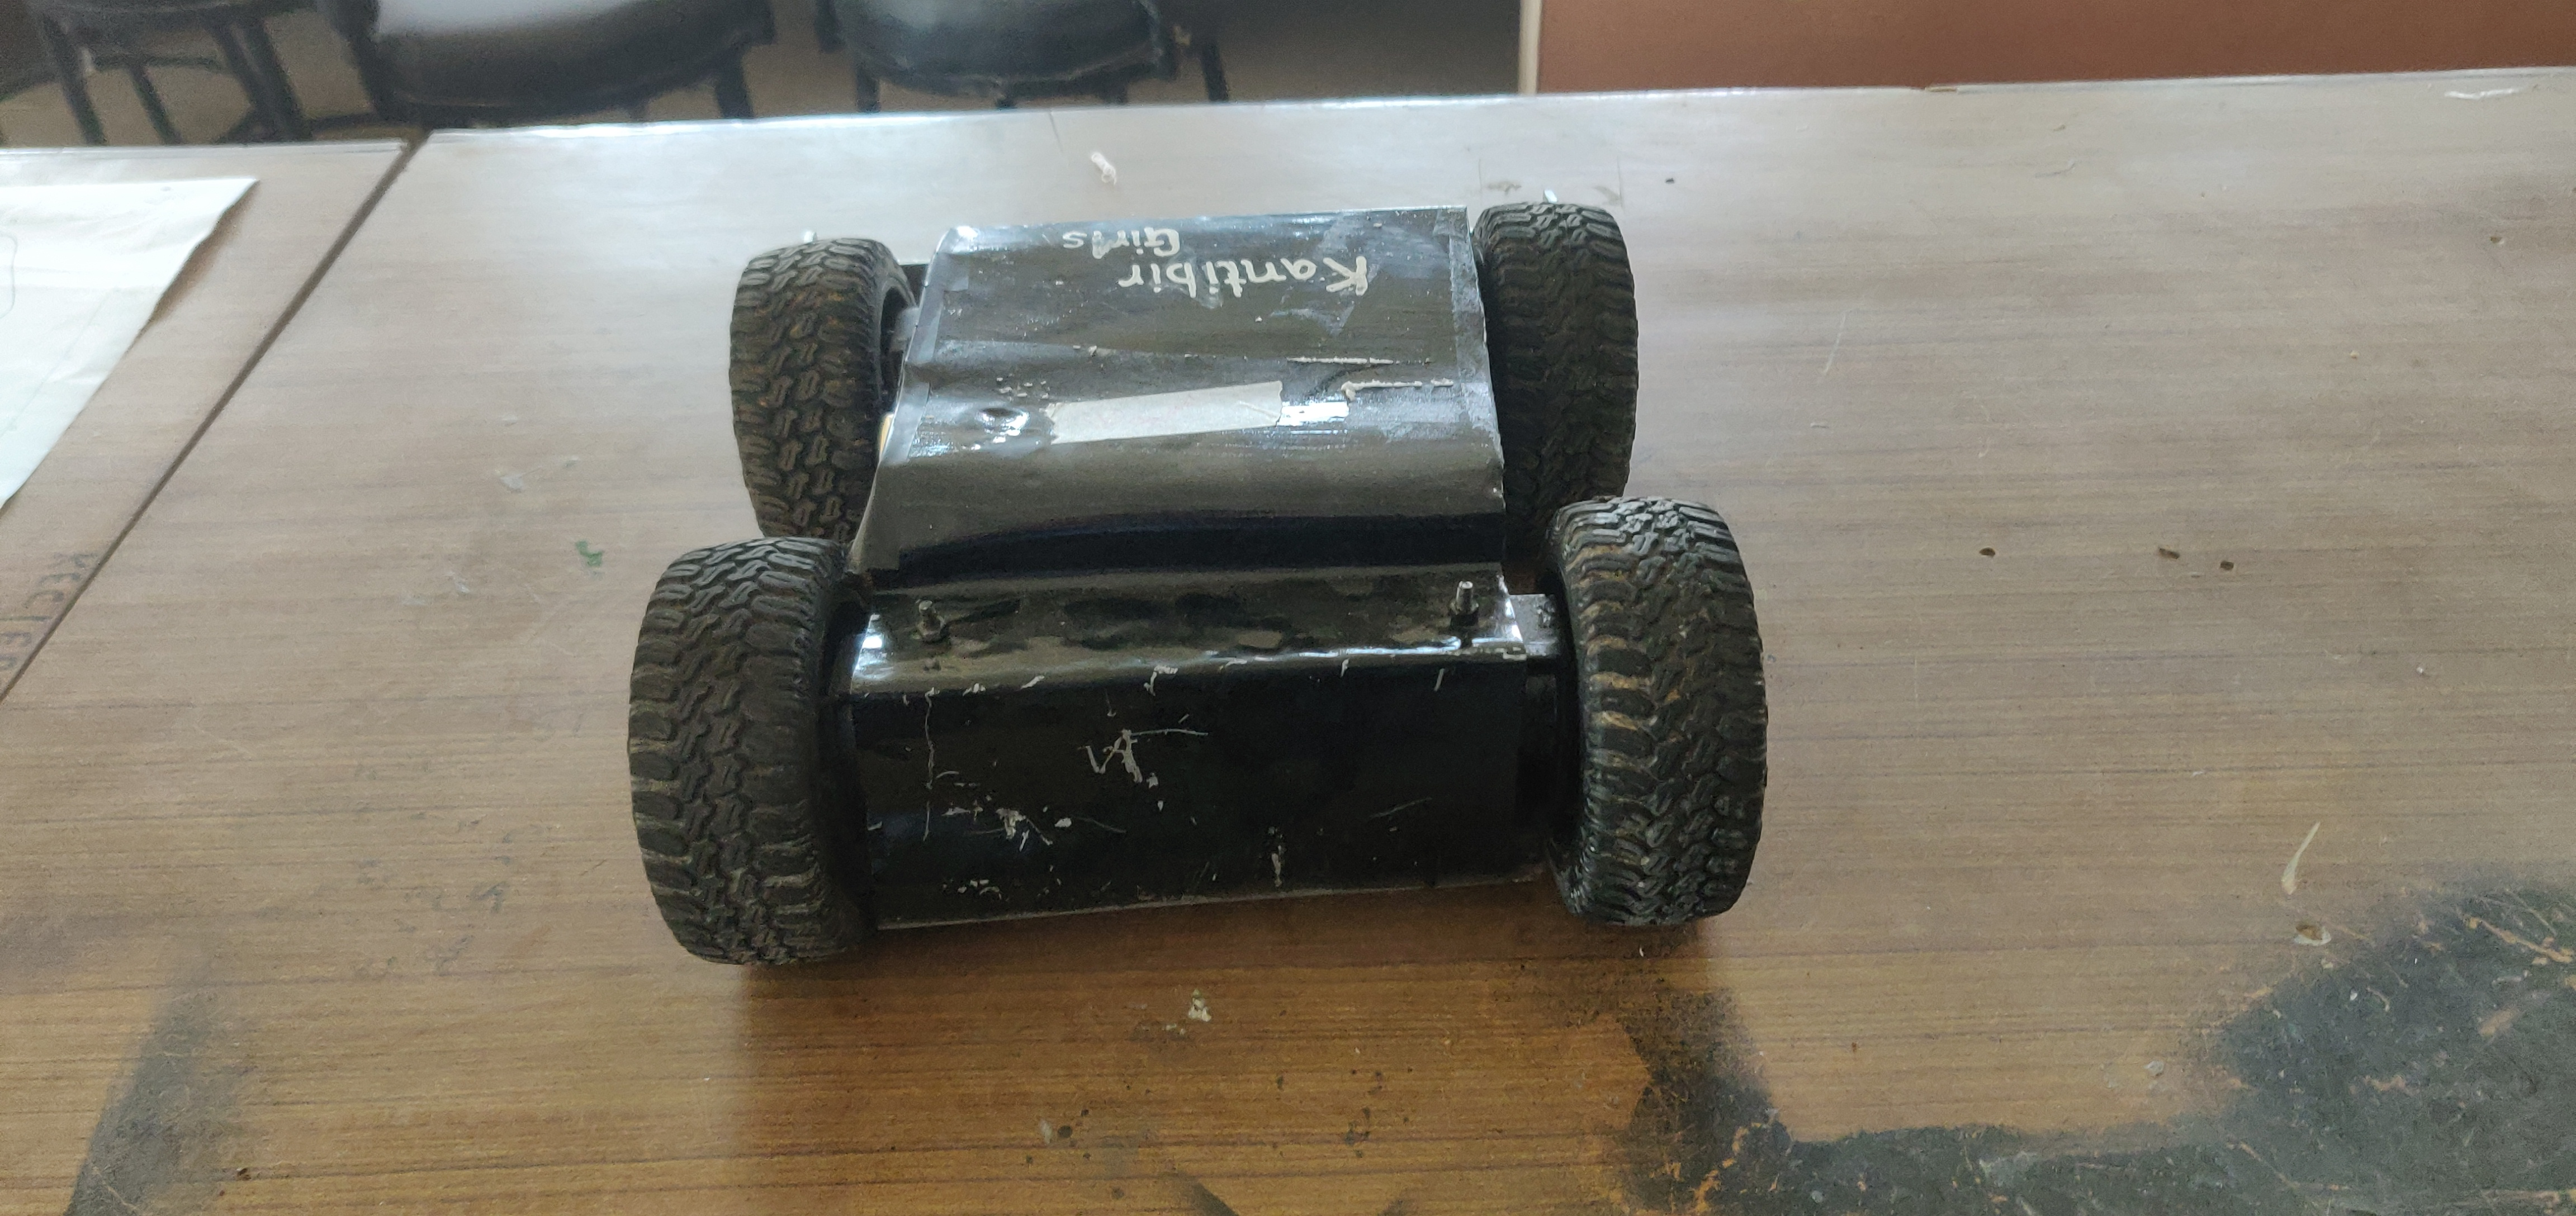
\includegraphics[width = 3in]{images/botpic11.jpg} 
	%\caption{Scaled Down Car } %figure name
	\label{figSample1} % for referencing
%\end{centre}
%\begin{centre}
	%
\includegraphics[width = 3in]{images/logo.png}
	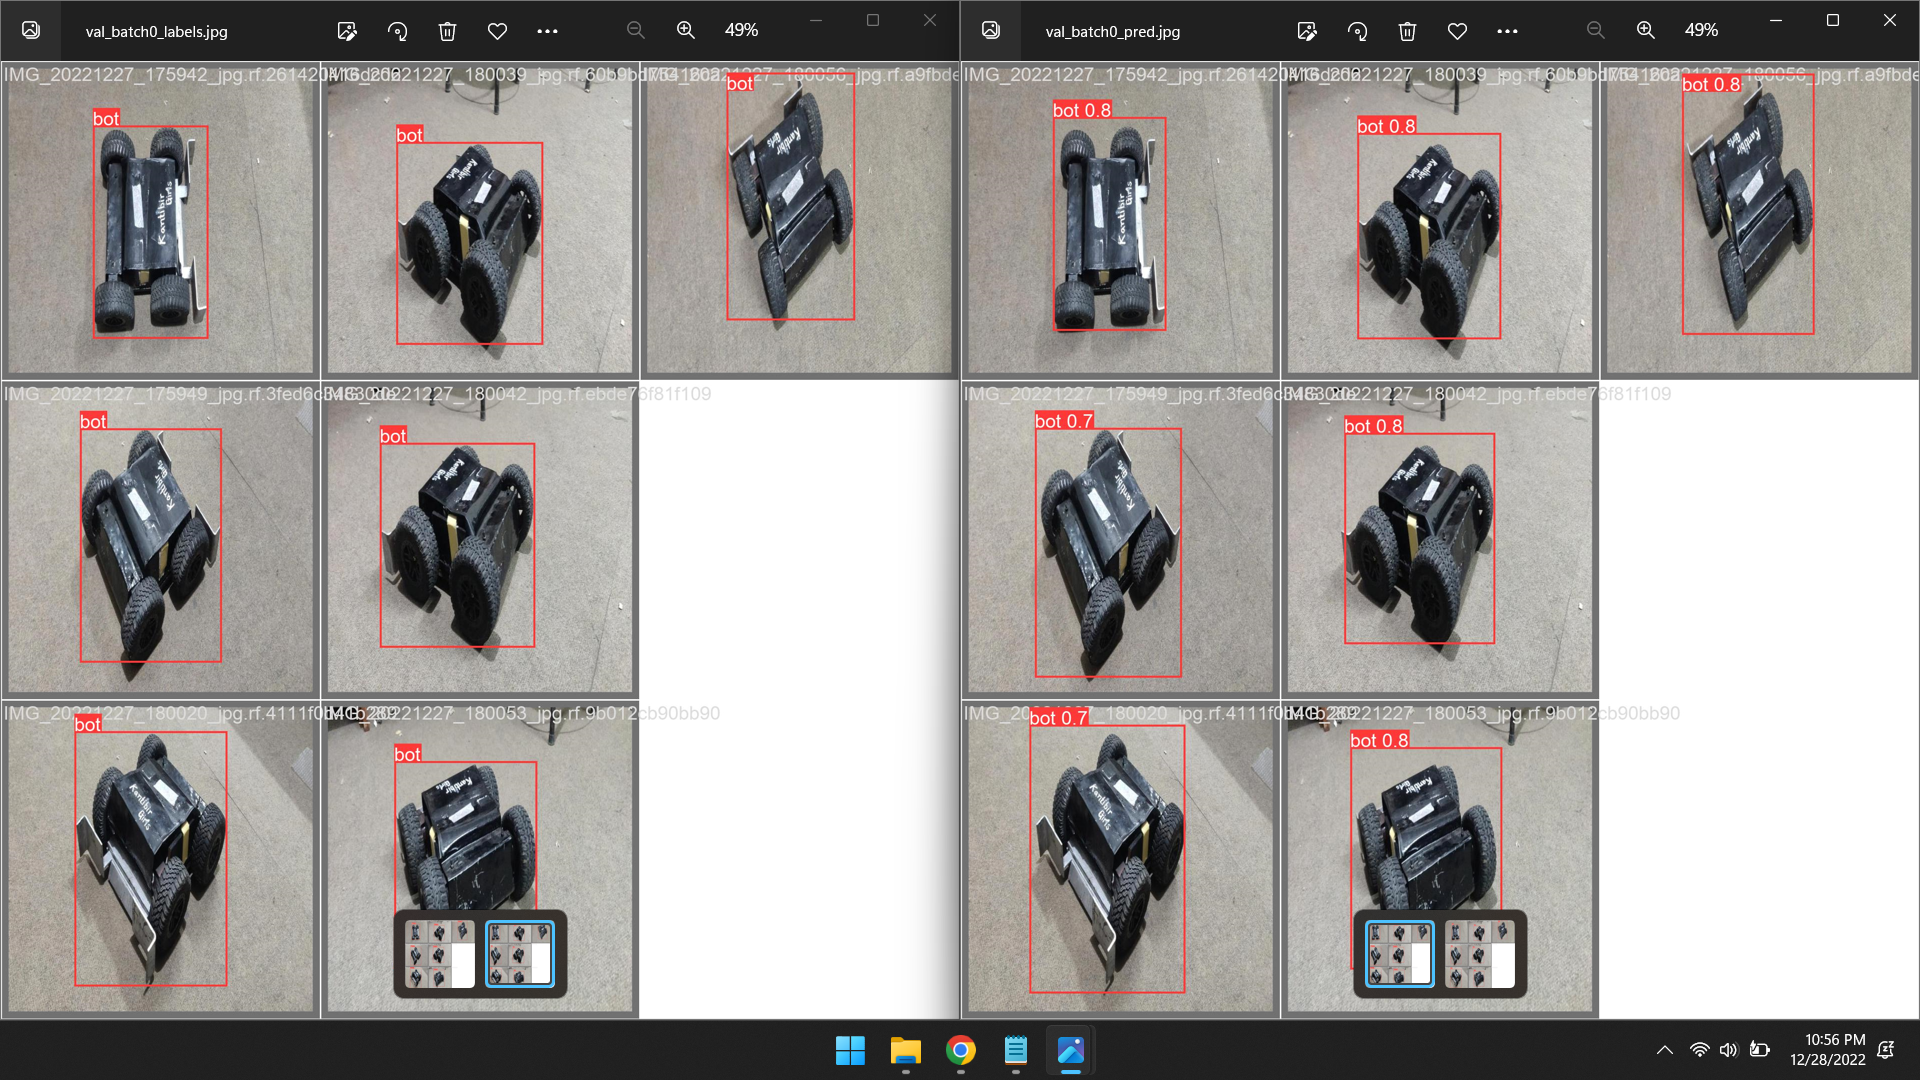
\includegraphics[width = 3in]{images/botlap.png} 
	\label{figSample1} % for referencing
%\end{centre}
\end{figure}


\begin{figure}[!tbh] % tbh means top, bottom or here (priority: left to right)
\%begin{center}
	%
\includegraphics[width = 3in]{images/logo.png}
	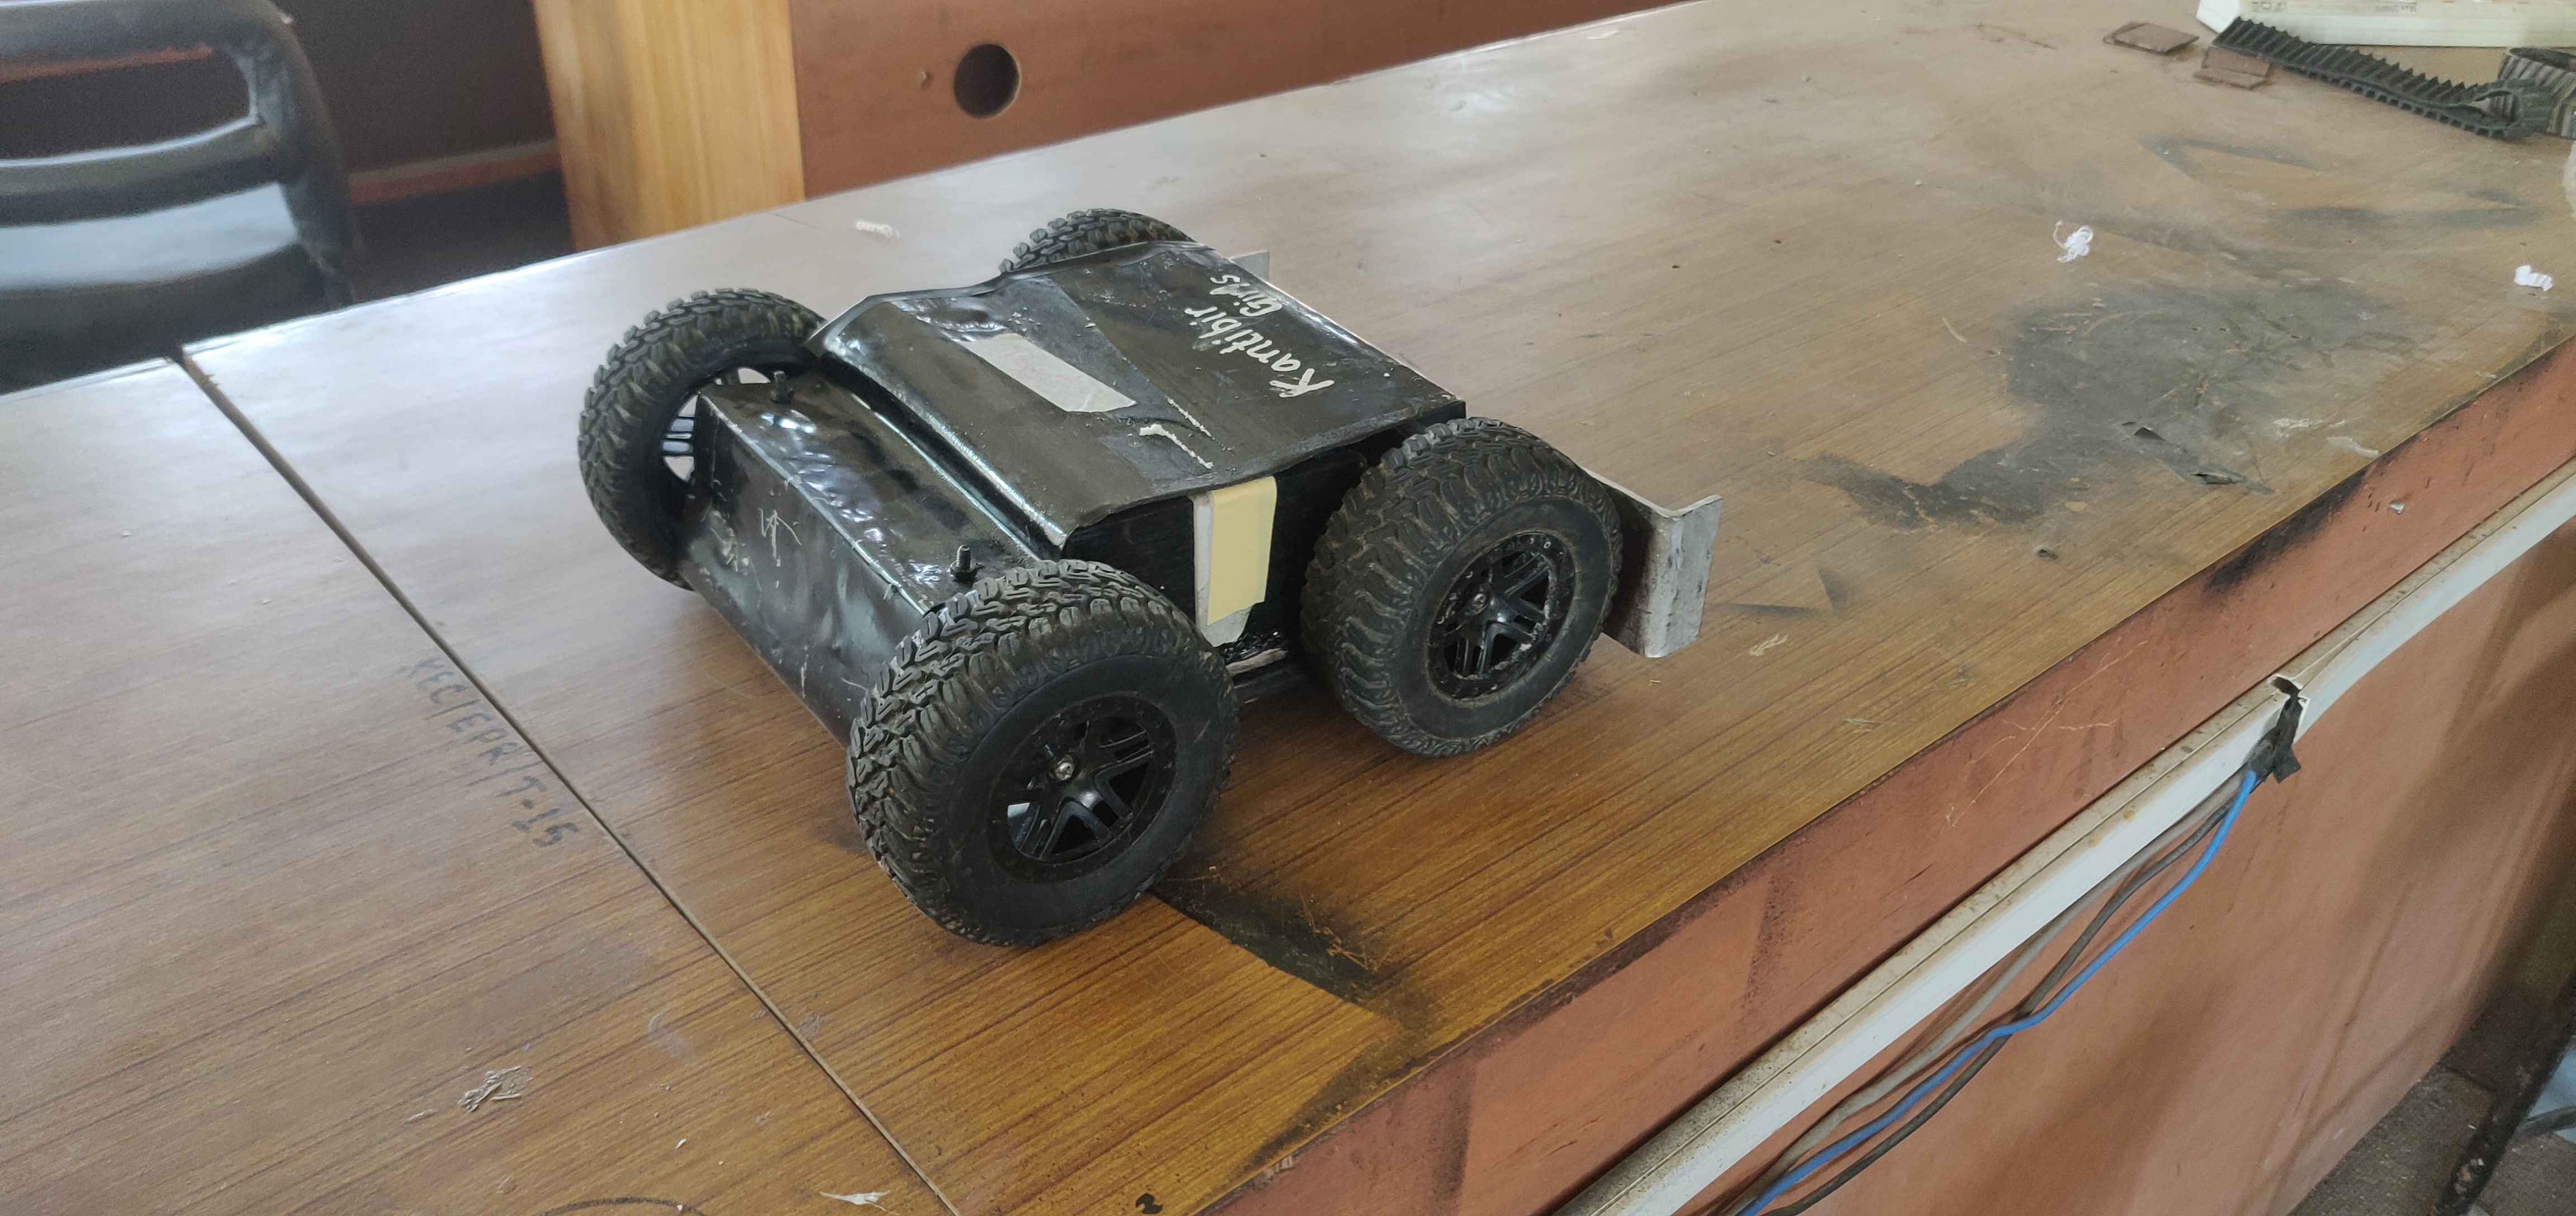
\includegraphics[width = 3in]{images/botpid7.jpg}
	\hspace{.5cm}
	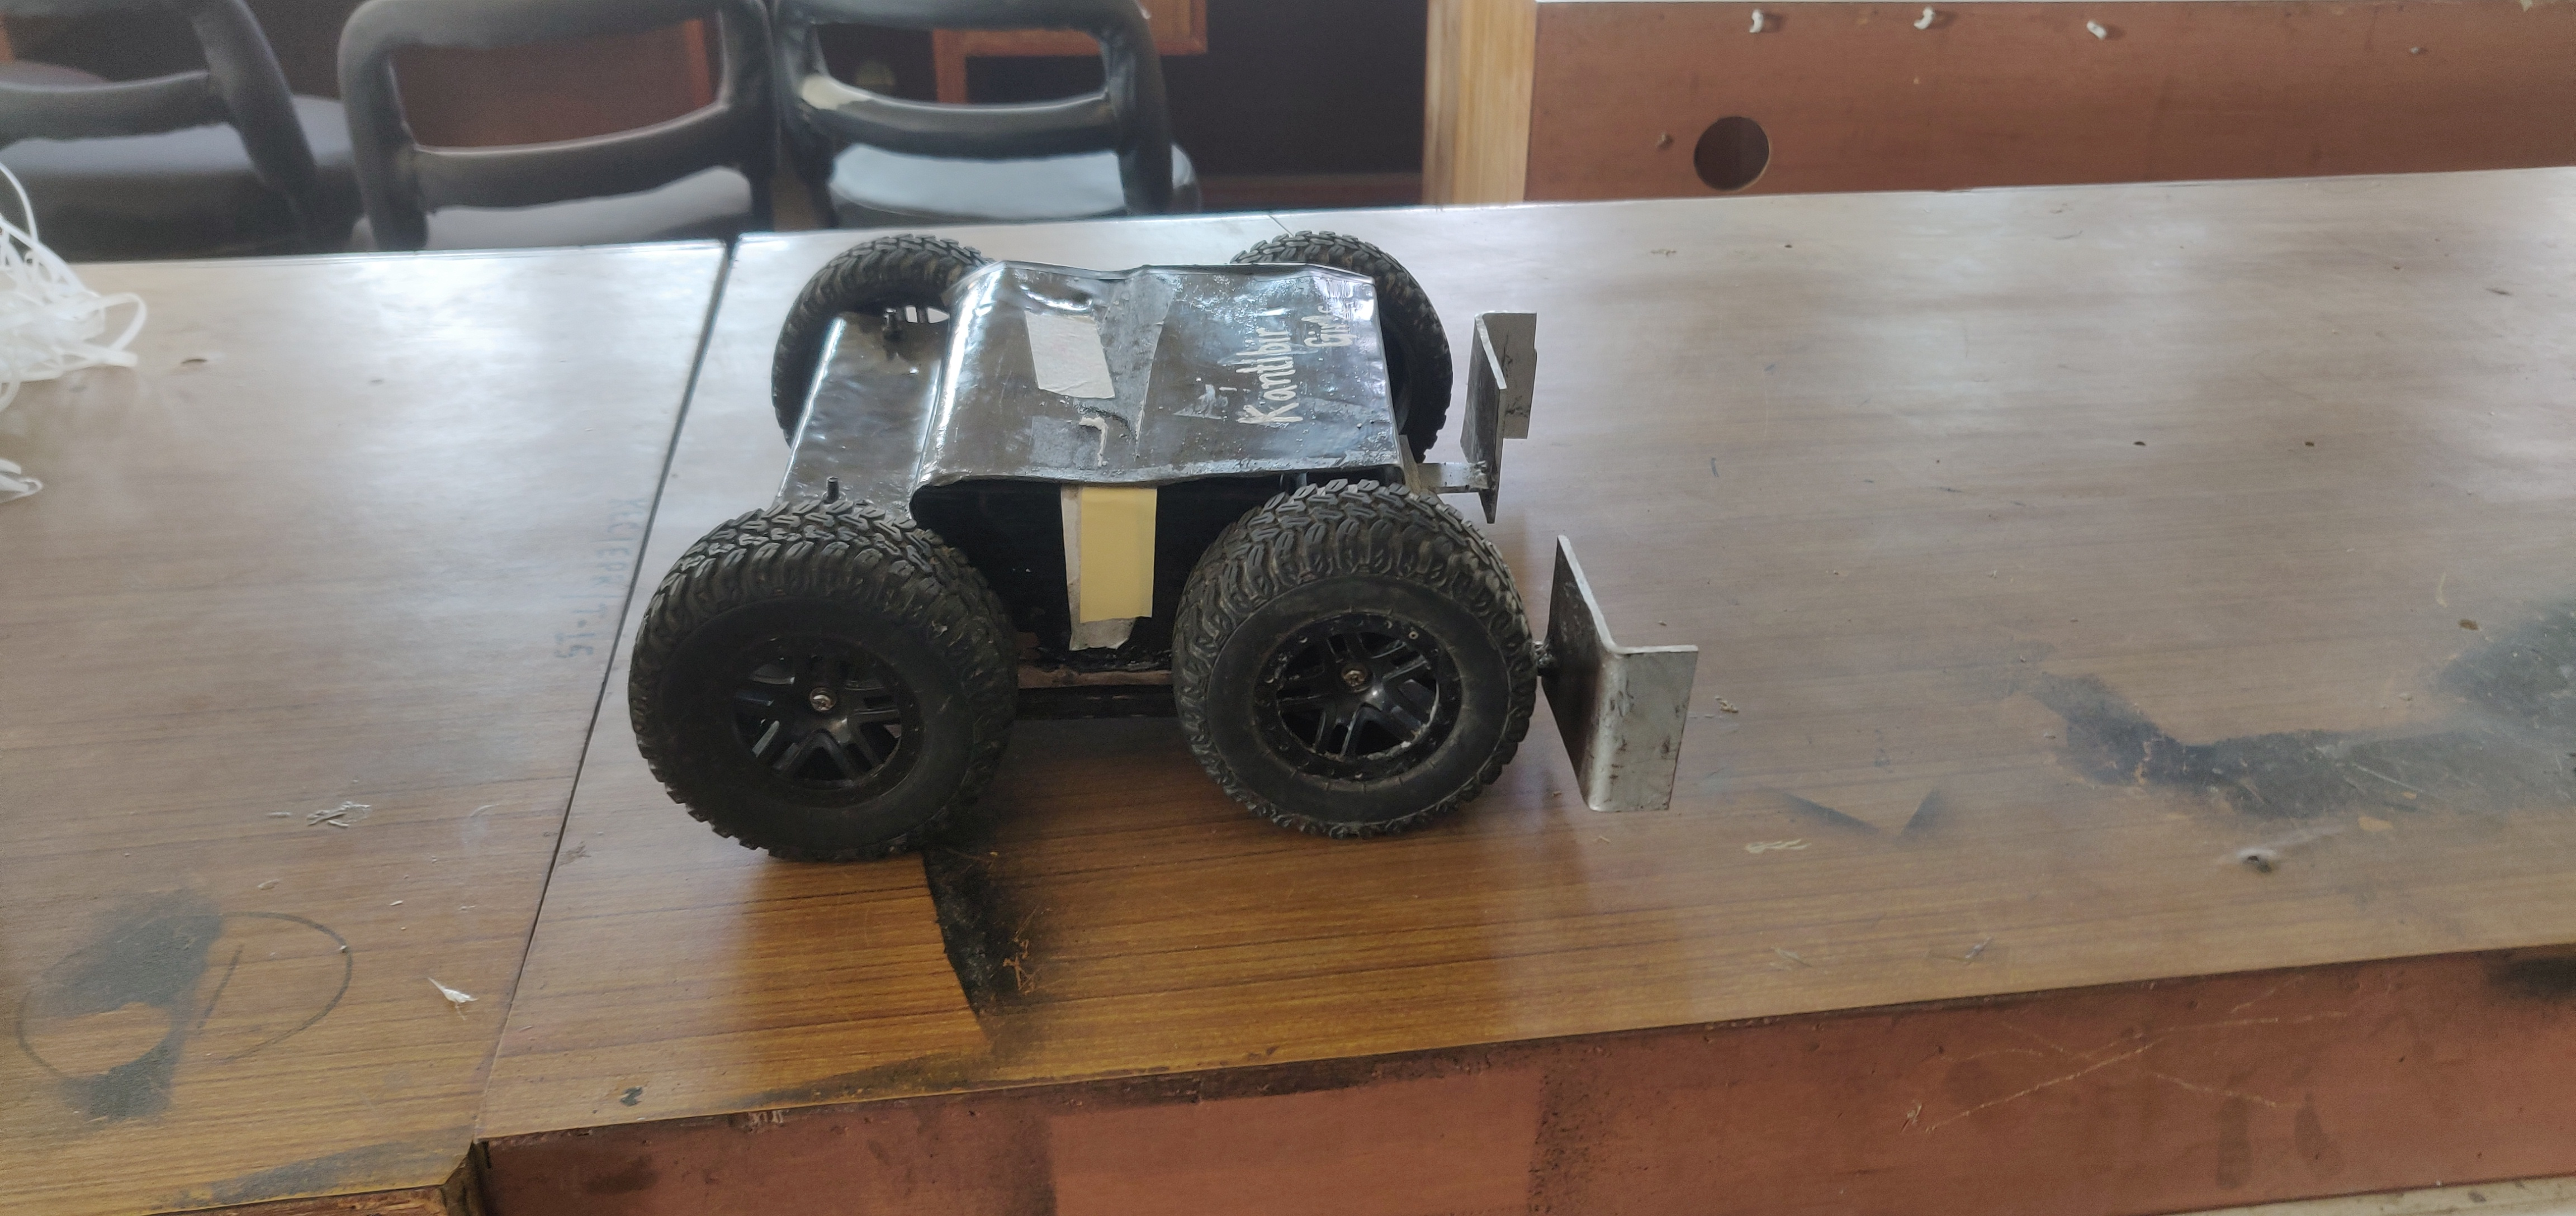
\includegraphics[width = 3in]{images/botpic8.jpg}
	%\caption{Scaled Down Car } %figure name
	\label{figSample1} % for referencing
%\end{centre}
\end{figure}



\subsubsection{Work in Process}
\begin{figure}[!tbh] % tbh means top, bottom or here (priority: left to right)
%\begin{centre}
	%
\includegraphics[width = 3in]{images/logo.png}
	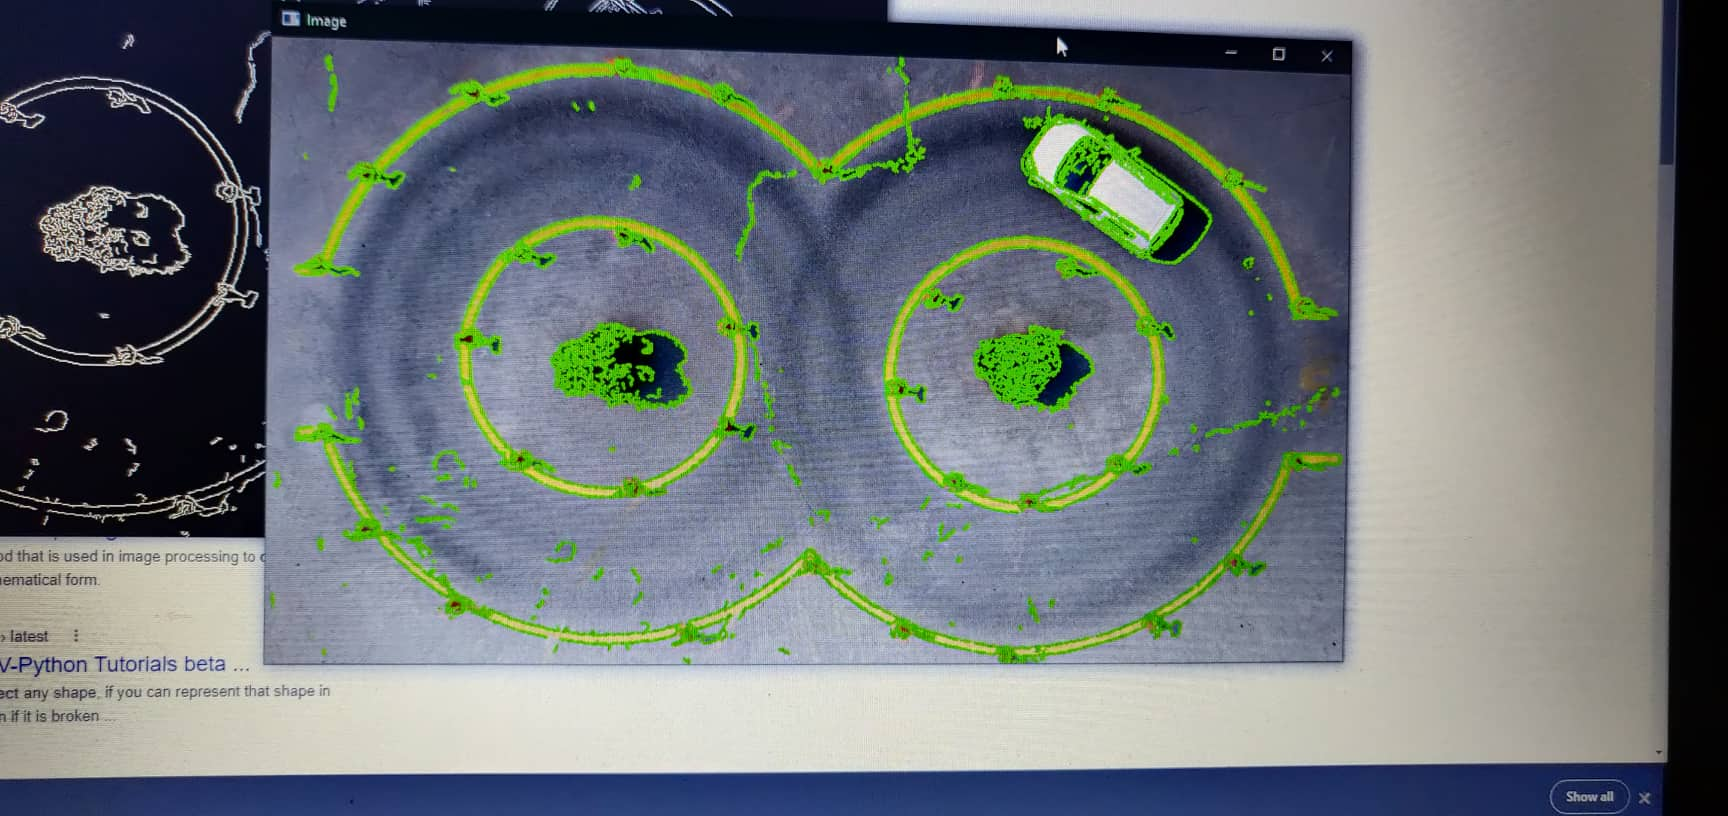
\includegraphics[width = 3in]{images/work in process1.jpg} 
	\hspace{.5cm}
	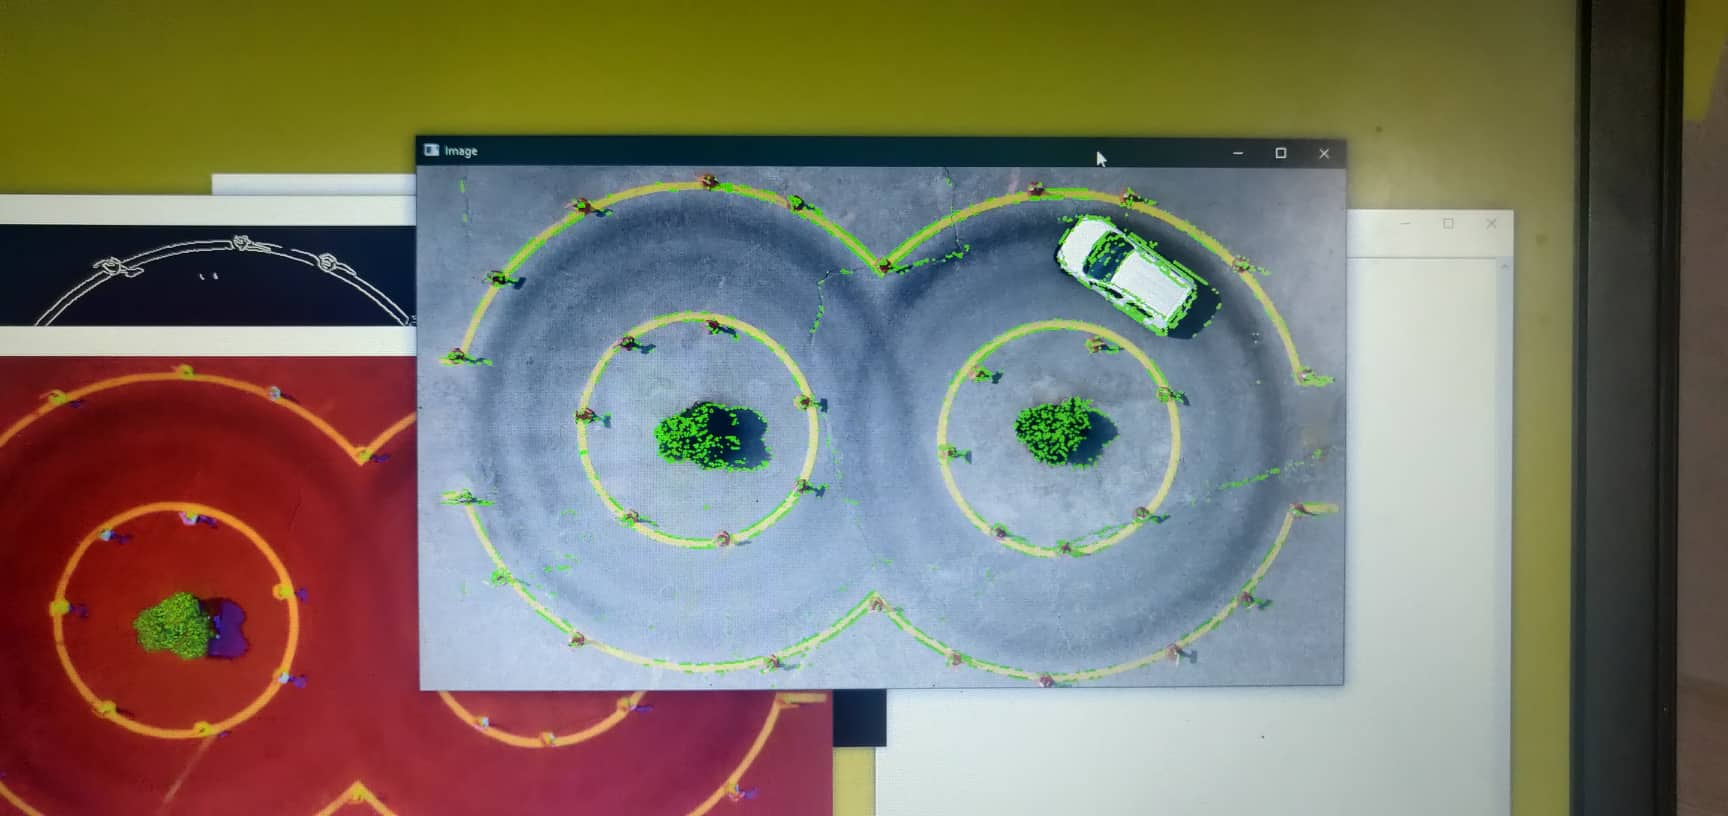
\includegraphics[width = 3in]{images/work in process2.jpg} 
	%\caption{Scaled Down Car } %figure name
	\label{figSample1} % for referencing
%\end{centre}
\end{figure}
\bibliography{reference.bib} % specify the .bib file containing reference information 
\renewcommand\bibname{References} % Change heading to References
\bibliographystyle{IEEEtr} % to use IEEE Format for referencing
\addcontentsline{toc}{chapter}{References} % to add references in TOC

\end{document}
